\newcommand{\DoNotLoadEpstopdf}{}
\documentclass[11pt]{article}
\ifdefined\pdfinfoomitdate\pdfinfoomitdate=1\fi
\ifdefined\pdftrailerid\pdftrailerid{}\fi
\usepackage[T1]{fontenc}
\usepackage{lmodern}
\usepackage[margin=1in]{geometry}
\usepackage{microtype}
\usepackage{amsmath,amssymb,amsthm,mathtools}
\usepackage{enumitem,booktabs,array}
\usepackage{tikz}
\usetikzlibrary{arrows.meta,positioning,decorations.pathreplacing,calc}
\usepackage{listings}
\usepackage[colorlinks=true,linkcolor=blue!55!black,citecolor=blue!55!black,urlcolor=blue!55!black]{hyperref}
\newtheorem{theorem}{Theorem}[section]
\newtheorem{lemma}[theorem]{Lemma}
\newtheorem{proposition}[theorem]{Proposition}
\newtheorem{corollary}[theorem]{Corollary}
\theoremstyle{definition}
\newtheorem{definition}[theorem]{Definition}
\newtheorem{remark}[theorem]{Remark}
\numberwithin{equation}{section}
\setlist{itemsep=3pt,topsep=5pt}
\lstset{basicstyle=\ttfamily\footnotesize,breaklines=true,columns=fullflexible,keepspaces=true,showstringspaces=false,frame=single,rulecolor=\color{black!20}}
\hypersetup{pdftitle={Cycle--clique Ramsey numbers},pdfauthor={OpenAI}}
\title{Cycle--clique Ramsey numbers}
\author{OpenAI}
\date{September 25, 2026}
\begin{document}
\maketitle
\begin{abstract}
We prove that $R(C_m,K_n)=(m-1)(n-1)+1$ for every pair of integers
$m\ge n\ge3$ other than $(m,n)=(3,3)$, for which $R(C_3,K_3)=6$.
This establishes the cycle--clique conjecture of Erd\H{o}s, Faudree,
Rousseau and Schelp. The proof combines expansion in a
minimal counterexample with a large-clique lemma and an optimization of
paths joining clique vertices. These arguments reduce the remaining cases
to $3{,}099$ finite parameter-pattern instances, which are excluded by two exact
implementations of proved inference rules. Complete programs and deduction
traces accompany the paper.
\end{abstract}
\tableofcontents
\section{Introduction}
\label{sec:introduction}

For finite simple graphs $H$ and $J$, the Ramsey number $R(H,J)$ is the
least integer $N$ such that every red--blue colouring of the edges of the
complete graph on $N$ vertices contains a red copy of $H$ or a blue copy of
$J$. Copies need not be induced. Write $C_m$ for the cycle on exactly $m$
vertices and $K_n$ for the complete graph on $n$ vertices.

\begin{theorem}\label{thm:main}
For all integers $m\ge n\ge3$ with $(m,n)\ne(3,3)$,
\[
 R(C_m,K_n)=(m-1)(n-1)+1.
\]
For the excluded pair, $R(C_3,K_3)=6$.
\end{theorem}

Theorem~\ref{thm:main} establishes the cycle--clique conjecture of
Erd\H{o}s, Faudree, Rousseau and Schelp
\cite{ErdosFaudreeRousseauSchelp1978}, in the formulation stated by
Keevash, Long and Skokan~\cite{KeevashLongSkokan2021}.
The cycle length in the theorem is exact. Its lower bound comes from
$n-1$ disjoint red cliques of order $m-1$, with all edges between them blue.
The task is to show that one additional vertex forces one of the two
specified graphs.

\subsection{Previous results and the parameter range}

The case $n=3$ goes back to Chartrand and Schuster
\cite{ChartrandSchuster1971}; see also Bondy and Erd\H{o}s
\cite[p.~47]{BondyErdos1973}. Bondy and Erd\H{o}s
\cite[Theorem~4]{BondyErdos1973} established the formula when
$m\ge n^2-2$. The complete conjectured range was established for $n=4$
by Yang, Huang and Zhang~\cite{YangHuangZhang1999}, for $n=5$ by
Bollob\'as and coauthors~\cite{BollobasEtAl2000}, for $n=6$ by
Schiermeyer~\cite{Schiermeyer2003}, and for $n=7$ by Chen, Cheng and
Zhang~\cite{ChenChengZhang2008}.
For $n=8$, further cases were established: $m=8$
\cite{JaradatAlzaleq2007,ZhangZhang2009}, $m=9$
\cite{BatainehJaradatAlZaleq2011}, and $10\le m\le15$
\cite{Baniabedalruhman2023}.
Theorem~1 of Nikiforov~\cite{Nikiforov2005} states the formula for
$n\ge4$ and $m\ge4n+2$.

Keevash, Long and Skokan~\cite[Theorem~1.1]{KeevashLongSkokan2021}
proved that an absolute constant $C\ge1$ suffices whenever
\begin{equation}\label{intro:kls}
 n\ge3,\qquad
 m\ge C\frac{\log_2 n}{\log_2\log_2 n}.
\end{equation}
This already contains every pair $m\ge n$ once $n$ is sufficiently large.
Indeed, the right-hand side of~\eqref{intro:kls} is $o(n)$.
For each of the finitely many smaller values of $n$, only finitely many
$m\ge n$ lie below that threshold. Thus their theorem leaves at most
finitely many pairs in the range of Theorem~\ref{thm:main}.
Our result completes that range. The finite calculation below comes from
an explicit structural reduction and does not require a numerical value
of the constant in~\eqref{intro:kls}.

\subsection{The proof}

Set $k=m-1$ and $a=n-1$. A failure of the upper bound gives a graph with
no cycle of order $k+1$ and independence number at most $a\le k$.
Holding $k$ fixed and minimizing $a$ produces a useful expansion property: every
nonempty independent set $I$ has at least $k|I|+1$ vertices in its closed
neighbourhood. In particular, the minimum degree is at least $k$.

The first structural step finds a clique of order
\[
 t\ge\max\{3,\lfloor k/2\rfloor\}.
\]
The proof uses distance layers in a rooted tree, followed by an explicit
path-rotation argument. Independent-set expansion and rooted distance
layers already appear in the cycle--clique argument of Erd\H{o}s,
Faudree, Rousseau and Schelp~\cite[Section~3]{ErdosFaudreeRousseauSchelp1978}.
We prove the particular quantitative statements needed here in
Sections~\ref{sec:reduction} and~\ref{sec:clique}.
The two smallest values $k=3,4$ are then settled directly.

For $k\ge5$, fix a maximum clique $Q$ of order $t$. Consider paths between
its vertices whose nonempty interiors lie outside $Q$ and are pairwise
disjoint, and whose endpoint pairs form disjoint chains. The total number
of interior vertices is called the \emph{amount} of the system. We maximize
this amount below $k+1-t$, breaking ties by minimizing the number of paths.
Certain improvements of this system would close to a cycle of order
exactly $k+1$; all such improvements are therefore forbidden.

These prohibitions make neighbourhoods of suitable path vertices
disjoint and anticomplete. Expansion then supplies independent sets
inside those neighbourhoods. A separate size lemma raises the available
independence bound from two to three when needed. For $t\ge9$, this
argument and a short numerical classification give more than $k$
independent vertices, a contradiction. Sections~\ref{sec:paths}--\ref{sec:terminal}
develop this part of the proof.

The remaining case has $3\le t\le8$, and the clique bound gives
$5\le k\le17$. A pattern records each chain by its sequence of
interior-vertex counts, up to chain reversal and permutation of components.
There are $3{,}099$ parameter-pattern instances across the $42$ admissible
pairs $(k,t)$. Section~\ref{sec:finite} proves the inference rules that
exclude them: path replacement, exact-cycle closure, neighbourhood
growth, independent-set packing, and contradiction under an added edge
or a path with one new interior vertex. The computation enumerates these
patterns, rather than graphs or edge colourings. Appendix~\ref{app:implementation}
describes two separate exact implementations and the accompanying
deduction traces. All structural arguments and all mathematical
inference rules are proved in the main text.

\section{A minimal counterexample and neighborhood expansion}
\label{sec:reduction}

All graphs in the proof are finite and simple. For a graph $H$, write
$\alpha(H)$ for its independence number, $\omega(H)$ for its clique
number, and $\delta(H)$ for its minimum degree. If $X\subseteq V(H)$,
then $H[X]$ is the induced subgraph on $X$ and $H-X$ is the induced
subgraph on $V(H)\setminus X$. We sometimes write $\alpha(X)$ for
$\alpha(H[X])$ when the ambient graph is clear. The open neighborhood
of a vertex $x$ is denoted by $N_H(x)$. For a set $X$, put
$N_H(X)=\bigcup_{x\in X}N_H(x)$, and
\[
  N_H[X]=X\cup\bigcup_{x\in X}N_H(x)
\]
is the closed neighborhood of a set $X$. Thus $N_H[x]=N_H[\{x\}]$.
The order of a path or cycle is its number of vertices, and its length
is its number of edges. In particular, a copy of $C_m$ always has
exactly $m$ vertices.

The upper bound is equivalent to the assertion that every graph on
$(m-1)(n-1)+1$ vertices contains either a cycle of order $m$ or an
independent set of order $n$: apply this assertion to the red graph of
a two-coloring. Set $k=m-1$ and $a=n-1$. In the range $m\ge n\ge3$
with $(m,n)=(3,3)$ excluded, these parameters satisfy
\[
  k\ge3,\qquad 2\le a\le k.
\]
Conversely, every such pair $(k,a)$ corresponds to a pair in the
required range. We will rule out counterexamples for each fixed $k$.

Fix $k\ge3$ and suppose that the upper bound fails for at least one
$a\in\{2,\ldots,k\}$. Choose the least such $a$, and fix a graph $G$
with
\begin{equation}
  |V(G)|=ka+1,\qquad \alpha(G)\le a,
  \qquad G\text{ contains no }C_{k+1}.
  \label{red:counterexample}
\end{equation}
The choice of the least independence parameter will turn deletion of
an independent set and all its neighbors into a useful expansion
bound. The graph $G$ and the parameter $k$ retain this meaning throughout
the upper-bound proof; the parameter $a$ is used through
Section~\ref{sec:small}.

\begin{lemma}\label{red:smaller}
For every integer $b$ with $0\le b<a$, a graph $H$ containing no
$C_{k+1}$ and satisfying $\alpha(H)\le b$ has at most $kb$ vertices.
\end{lemma}

\begin{proof}
If $b=0$, the graph $H$ is empty, since any vertex would be an
independent set of order one. If $b=1$, the graph is complete. A
complete graph with at least $k+1$ vertices contains a cycle of exactly
$k+1$ vertices, so in this case $|V(H)|\le k$.

Now let $2\le b<a$. If $|V(H)|\ge kb+1$, take an induced subgraph on
$kb+1$ vertices. It still contains no $C_{k+1}$ and has independence
number at most $b$. It would therefore be a counterexample for the
smaller parameter $b$, contrary to the choice of $a$.
\end{proof}

Independent-set deletion and neighbourhood expansion already enter the
cycle--clique argument of Erd\H{o}s, Faudree, Rousseau and Schelp
\cite[Section~3]{ErdosFaudreeRousseauSchelp1978}. The following closed
neighbourhood bound comes directly from our fixed-parameter minimality.

\begin{lemma}[Independent-set expansion]\label{red:expansion}
For every nonempty independent set $I$ in the graph $G$ fixed in
\eqref{red:counterexample},
\begin{equation}
  |N_G[I]|\ge k|I|+1.
  \label{red:expansion-bound}
\end{equation}
In particular, $\delta(G)\ge k$ and $\alpha(G)\le k$.
\end{lemma}

\begin{proof}
Put $r=|I|$, so that $1\le r\le a$. Every independent set in
$G-N_G[I]$ can be adjoined to $I$, because it has no edges to $I$.
Consequently,
\[
  \alpha\bigl(G-N_G[I]\bigr)\le a-r.
\]
The integer $a-r$ lies between zero and $a-1$. The graph
$G-N_G[I]$ also contains no $C_{k+1}$, so Lemma~\ref{red:smaller}
applies, including when $r=a$, and gives
\[
  |V(G)\setminus N_G[I]|\le k(a-r).
\]
Subtracting from $|V(G)|=ka+1$ proves
\eqref{red:expansion-bound}. Applying the bound to $I=\{x\}$ yields
$d_G(x)+1\ge k+1$, and hence $\delta(G)\ge k$. Finally,
$\alpha(G)\le a\le k$ by the choice of the parameters.
\end{proof}

The remainder of the upper-bound proof uses
\eqref{red:counterexample} and Lemma~\ref{red:expansion} to derive a
contradiction. The first structural step, in
Section~\ref{sec:clique}, finds a large clique. Section~\ref{sec:small}
then disposes of $k=3,4$; all later arguments may assume $k\ge5$.

\section{A large clique}\label{sec:clique}

We continue with the graph from Section~\ref{sec:reduction}, and write
\(t=\omega(G)\) for its maximum clique size.  The next result supplies the
clique around which we will organize the rest of the proof.

\begin{theorem}\label{clq:bound}
Let \(k\ge3\) and \(2\le a\le k\) be integers, and let \(G\) be a finite
simple graph such that
\[
 |V(G)|=ka+1,\qquad \alpha(G)\le a,\qquad C_{k+1}\not\subseteq G.
\]
Suppose also that
\[
 |N_G[I]|\ge k|I|+1
 \quad\text{for every nonempty independent set }I\subseteq V(G).
\]
Then its maximum clique size \(t\) satisfies
\begin{equation}\label{clq:bound-equation}
 \max\{3,\lfloor k/2\rfloor\}\le t\le k.
\end{equation}
\end{theorem}

Lemma~\ref{red:expansion} gives the expansion hypothesis for our graph.
We first obtain a triangle.  For larger \(k\), we then find an induced
subgraph in a single distance layer with enough internal expansion to
force a long path.  Tree paths above that layer will close the path into
a cycle on exactly \(k+1\) vertices. This layer-and-tree strategy has its
antecedent in Erd\H{o}s, Faudree, Rousseau and Schelp
\cite[Section~3]{ErdosFaudreeRousseauSchelp1978}; the quantitative layer
and coloured-path statements used here are proved below.

\begin{lemma}\label{clq:triangle}
Under the hypotheses of Theorem~\ref{clq:bound}, we have \(3\le t\le k\).
\end{lemma}

\begin{proof}
A clique on \(k+1\) vertices contains a \(C_{k+1}\), so \(t\le k\).
For the other inequality, put \(r_b=R(K_3,K_b)\).  The elementary
Ramsey recurrence gives
\[
 r_2=3,\qquad r_b\le b+r_{b-1}\quad(b\ge3),
 \qquad r_b\le\frac{b(b+1)}2.
\]
Indeed, in a graph on \(b+r_{b-1}\) vertices, choose a vertex \(v\).
If \(v\) has at least \(b\) neighbors, either two of them are adjacent,
giving a triangle, or there is an independent set of size \(b\).
Otherwise \(v\) has at least \(r_{b-1}\) nonneighbors; among them there
is a triangle or an independent set of size \(b-1\), to which \(v\)
can be added.  Induction gives the displayed bound on \(r_b\).

Since \(a\le k\) and \(k\ge3\), we have \(a+3\le2k\), and hence
\[
 R(K_3,K_{a+1})\le\frac{(a+1)(a+2)}2\le ka+1=|V(G)|.
\]
The alternative of an independent set of size \(a+1\) is excluded,
so \(G\) contains a triangle.
\end{proof}

For \(k\le7\), Lemma~\ref{clq:triangle} already proves
Theorem~\ref{clq:bound}.  We therefore consider \(k\ge8\), and put
\(s=\lfloor k/2\rfloor\ge4\).  The following proposition isolates
the information needed from the distance layers.  It does not require
the whole graph to be connected.

\begin{proposition}\label{clq:layer-interface}
Let \(k\ge8\) be an integer, set \(s=\lfloor k/2\rfloor\), and let \(G\) be a
nonempty finite simple graph with \(\alpha(G)\le k\) and
\[
 |N_G[I]|\ge k|I|+1
 \quad\text{for every nonempty independent set }I\subseteq V(G).
\]
Suppose that \(G\) contains no \(K_s\).  Fix a vertex \(r\) and a
breadth-first spanning tree \(T\) of its component, rooted at \(r\).
Then there exist \(i\in\{1,\ldots,s\}\) and an induced subgraph \(H\)
of \(G\), all of whose vertices have depth \(i\) in \(T\), such that
\(H\) is connected and nonbipartite, and
\begin{equation}\label{clq:H-properties}
 \begin{gathered}
 |V(H)|\ge k,\qquad \delta(H)\ge s,\\
 |N_H[I]|\ge s|I|
 \quad(I\ne\varnothing\text{ independent in }H).
 \end{gathered}
\end{equation}
The last inequality is strict whenever \(k\) is odd or
\(H-N_H[I]\) is nonempty.
\end{proposition}

\begin{proof}
Let \(D_j\) be the set of vertices at distance \(j\) from \(r\).
These are exactly the depth layers of \(T\).  Layers beyond the
maximum depth are empty, and we use \(\alpha(\varnothing)=0\).
Every edge in the root component joins layers whose indices differ
by at most one.  Thus maximum independent sets chosen in layers of
one parity can be united, giving an independent set of size
\[
 p_i:=\sum_{\substack{0\le j\le i\\j\equiv i\pmod2}}
             \alpha(D_j).
\]
In particular \(p_i\le k\) and \(p_0=1\).  Applying expansion to a
singleton gives \(\delta(G)\ge k\), so \(D_1\ne\varnothing\).
Consequently every union defining \(p_i\) is nonempty: it contains
either the root or an independent vertex from \(D_1\).

For \(1\le i\le s\), the closed neighborhood of the independent
union defining \(p_{i-1}\) is contained in
\(D_0\cup\cdots\cup D_i\).  No vertex in another component is
adjacent to this union.  Expansion and \(|D_0|=1\) give
\begin{equation}\label{clq:layer-sum}
 \sum_{j=1}^i|D_j|\ge kp_{i-1}.
\end{equation}
Also, the two parity sums partition the indices from zero through
\(i\), so
\begin{equation}\label{clq:parity-sum}
 \sum_{j=1}^i\alpha(D_j)=p_i+p_{i-1}-1.
\end{equation}

Suppose first that \(k=2s\).  If every nonempty layer \(D_j\),
\(1\le j\le s\), satisfied \(|D_j|<s\alpha(D_j)\), then
\eqref{clq:layer-sum} and \eqref{clq:parity-sum} would imply
\[
 2sp_{i-1}\le\sum_{j=1}^i|D_j|
   <s(p_i+p_{i-1}-1)\qquad(1\le i\le s).
\]
The strict inequality holds even when some layers are empty, since
every sum contains the nonempty layer \(D_1\).
It follows that \(p_i>p_{i-1}+1\), and therefore, by integrality,
\(p_i\ge p_{i-1}+2\).  Iterating to \(i=s\) gives
\(p_s\ge2s+1>k\), a contradiction.  Hence some nonempty layer
\(D_i\), \(1\le i\le s\), satisfies
\begin{equation}\label{clq:even-layer}
 |D_i|\ge s\alpha(D_i).
\end{equation}

Now suppose that \(k=2s+1\).  If \(|D_j|\le s\alpha(D_j)\) for
every \(1\le j\le s\), including empty layers, the same two
identities give
\[
 (2s+1)p_{i-1}\le s(p_i+p_{i-1}-1),
 \qquad
 p_i\ge p_{i-1}+1+\left\lceil\frac{p_{i-1}}s\right\rceil.
\]
Starting from \(p_0=1\), each increment is at least two, so
\(p_{s-1}\ge2s-1>s\).  The last increment is consequently at least
three, giving \(p_s\ge2s+2>k\), again a contradiction.  Thus some
layer \(D_i\), \(1\le i\le s\), satisfies
\begin{equation}\label{clq:odd-layer}
 |D_i|>s\alpha(D_i).
\end{equation}
This layer is necessarily nonempty.

We have found a layer of sufficiently large order relative to its
independence number.  Choose within it a nonempty induced subgraph
\(H\) of minimum order satisfying the corresponding inequality
\eqref{clq:even-layer} or \eqref{clq:odd-layer}.  Since \(G\) has
no \(K_s\), such an \(H\) cannot be complete: a complete graph
satisfying either inequality would have at least \(s\) vertices.
Thus \(\alpha(H)\ge2\).  For even \(k\) this gives
\(|V(H)|\ge2s=k\); for odd \(k\) it gives
\(|V(H)|>2s\), hence \(|V(H)|\ge2s+1=k\).

The graph \(H\) is connected.  Otherwise each component \(H_j\)
would be a proper nonempty induced subgraph and would fail the
chosen inequality.  Since independence number is additive across
components, summing these failures would give
\[
 \begin{cases}
 |V(H)|<s\alpha(H),&k\text{ even},\\
 |V(H)|\le s\alpha(H),&k\text{ odd},
 \end{cases}
\]
contrary to its choice.  Nor is \(H\) bipartite: a bipartition
would give \(\alpha(H)\ge |V(H)|/2\), incompatible with
\(|V(H)|\ge s\alpha(H)\) and \(s\ge4\).

Let \(I\) be a nonempty independent set in \(H\), and put
\(R=H-N_H[I]\).  An independent set in \(R\) can be united with
\(I\), so
\[
 \alpha(R)\le\alpha(H)-|I|.
\]
If \(R\ne\varnothing\), minimality gives
\(|V(R)|<s\alpha(R)\) for even \(k\), and
\(|V(R)|\le s\alpha(R)\) for odd \(k\).  Comparing with the
defining inequality for \(H\), one comparison is strict in each
parity.  Therefore
\[
 |N_H[I]|=|V(H)|-|V(R)|
   >s\bigl(\alpha(H)-\alpha(R)\bigr)\ge s|I|.
\]
If \(R=\varnothing\), instead use
\(|N_H[I]|=|V(H)|\ge s\alpha(H)\ge s|I|\); the first
inequality is strict for odd \(k\).

Finally, take \(I=\{v\}\).  When \(H-N_H[v]\) is nonempty, the
strict neighborhood bound gives \(d_H(v)+1>s\), hence
\(d_H(v)\ge s\).  When it is empty, the order bound gives
\(d_H(v)=|V(H)|-1\ge k-1\ge s\).  This proves all the asserted
properties of \(H\).
\end{proof}

We now have a connected, nonbipartite graph \(H\) inside a single
depth layer \(D_i\), with \(1\le i\le s\), satisfying
\eqref{clq:H-properties}.  Under the assumption that \(G\) has no
\(K_s\), the same is true of \(H\).  The next argument uses these
properties to construct a path in \(H\) whose ends can be joined
through the tree above \(D_i\), producing the forbidden cycle.

\subsection{Paths of a prescribed length}

We now show how the graph supplied by
Proposition~\ref{clq:layer-interface} yields a forbidden cycle.
The main step concerns paths whose ends lie in different parts of a
partition.  We first record the elementary longest-path bound needed
when all vertices of the layer have a common tree parent.

\begin{lemma}\label{clq:long-path}
Let $d\ge 2$, and let $F$ be a finite connected graph with
$\delta(F)\ge d$.  Then $F$ contains a path of order at least
$\min\{|V(F)|,2d+1\}$.
\end{lemma}

\begin{proof}
Let $v_1,\ldots,v_r$ be a longest path in $F$.  All neighbors of either
end belong to the path.  Suppose that
$r<\min\{|V(F)|,2d+1\}$.  The two sets
\[
 \{j\in\{1,\ldots,r-1\}:v_jv_r\in E(F)\},\qquad
 \{j\in\{1,\ldots,r-1\}:v_1v_{j+1}\in E(F)\}
\]
have at least $d$ elements each, whereas their common index set has
$r-1\le 2d-1$ elements.  Choose an index $j$ in their intersection.
If $j=1$ or $j=r-1$, the edge $v_1v_r$ closes the path to a cycle.
For $2\le j\le r-2$, the two indicated edges instead give the cycle
\[
 v_1,\ldots,v_j,v_r,v_{r-1},\ldots,v_{j+1},v_1
\]
through all vertices of the path.  Thus in every case there is a
cycle on these $r$ vertices.
Since $r<|V(F)|$ and $F$ is connected, some vertex outside the cycle
has a neighbor on it.  Starting with that vertex and then traversing
the cycle with one edge omitted gives a longer path, a contradiction.
\end{proof}

The next lemma uses only minimum degree, the exclusion of a clique,
and expansion of independent pairs.  Its proof identifies a clique of
possible path ends, shows that this clique attaches to the remaining
graph through one vertex, and uses that attachment to extend a path.

\begin{lemma}\label{clq:coloured-path}
Let $s\ge 4$, and let $H$ be a finite connected nonbipartite graph
containing no $K_s$.  Suppose that
\[
 \delta(H)\ge s,
 \qquad
 |N_H[\{a,b\}]|\ge 2s
 \quad\text{whenever $a,b$ are distinct and nonadjacent.}
\]
For every nonconstant map $\chi:V(H)\to\{0,1\}$ and every integer
$1\le\ell\le 2s-2$, there is a path in $H$ of length exactly $\ell$
whose ends receive different values of $\chi$.
\end{lemma}

\begin{proof}
Fix $\chi$ and $\ell$, and suppose that no such path exists.
There are vertices $y,z$ with $\chi(y)\ne\chi(z)$ and a common
neighbor $x$.  Indeed, if no such pair existed, the color would be
preserved along every walk of length two.  In a connected nonbipartite
graph there is an even walk between any two vertices: if a connecting
path has odd length, first insert an odd closed walk obtained by going
to an odd cycle, traversing it, and returning.  Preservation of the
color along successive pairs of steps would make $\chi$ constant.
This proves the assertion, and $x,y,z$ are distinct because the graph
is simple.

Let $K$ be the component containing $x$ in $H-\{y,z\}$.
Every vertex of $K$ loses at most two neighbors on deleting $y,z$,
and all its other neighbors lie in the same component.  Thus
\begin{equation}\label{clq:component-degree}
 \delta(K)\ge s-2.
\end{equation}
There is no path of order at least $\ell$ starting at $x$ in $K$.
For the first $\ell$ vertices of such a path form a path with some
last vertex $b$.  At least one of $y,z$ has color different from $b$;
prefixing that vertex gives a path of length $\ell$ with differently
colored ends.

Choose a longest path $P$ starting at $x$ in $K$, and write
$W=V(P)$ and $r=|W|$.  All neighbors in $K$ of its last vertex lie
on $P$, so \eqref{clq:component-degree} gives $r\ge s-1$.
If $\ell\le s-1$, this already contradicts the preceding paragraph.
This disposes in particular of $\ell=1,2$.  Henceforth we have
\begin{equation}\label{clq:path-order}
 s\le\ell\le 2s-2,
 \qquad s-1\le r\le\ell-1.
\end{equation}

\medskip
\noindent\emph{The possible last vertices form a clique.}
Define
\[
 E=\{e\in W:\text{there is a path from $x$ to $e$
 whose vertex set is exactly $W$}\}.
\]
Every such path has the maximum possible order among paths starting
at $x$ in $K$.  Its last vertex has no neighbor in $K-W$.
Since vertices of $K$ have no neighbors in
$H-(K\cup\{y,z\})$, we obtain
\begin{equation}\label{clq:endpoint-neighbors}
 N_K(e)\subseteq W,
 \qquad N_H(e)\subseteq W\cup\{y,z\}
 \quad(e\in E).
\end{equation}
If two vertices of $E$ were nonadjacent, their closed neighborhood
in $H$ would have size at most
$r+2\le\ell+1\le 2s-1$, contrary to the hypothesis.
Thus $E$ is a clique.  Also $x\notin E$, because a simple path with
more than one vertex has distinct ends, and $r\ge s-1\ge3$.

We use the standard fixed-end path rotation of P\'osa
\cite[p.~358]{Posa1963}. The endpoint-clique and attachment conclusions
needed here follow from our stated hypotheses. Explicitly, let
$v_1=x,\ldots,v_r=e$ be any path from $x$ with vertex set $W$.
For an edge $ev_j$ with $1\le j\le r-2$, the sequence
\begin{equation}\label{clq:rotation}
 v_1,\ldots,v_j,v_r,v_{r-1},\ldots,v_{j+1}
\end{equation}
is another path from $x$ on exactly $W$.  Its last vertex is
$v_{j+1}$.  The operation is valid also when $j=1$, so the pivot
may be $x$.  For $j=r-1$, the original path itself has last vertex
$v_{j+1}=e$.  Therefore the successor of every neighbor of $e$
along the path belongs to $E$.  Different neighbors have different
successors, and hence
\begin{equation}\label{clq:endpoint-degree}
 d_K(e)\le |E| \qquad(e\in E).
\end{equation}
Combining \eqref{clq:component-degree} with the fact that $E$ is a
clique and $H$ has no $K_s$ gives
\begin{equation}\label{clq:endpoint-size}
 s-2\le |E|\le s-1.
\end{equation}

On every path from $x$ with vertex set $W$, the vertices of $E$ form
a consecutive final segment.  To see this, let $e$ be its last
vertex.  Every earlier vertex of $E$ is adjacent to $e$, since $E$
is a clique.  The rotation then places its successor in $E$ as well.
Thus membership in $E$ is preserved on moving forward along the path.

\medskip
\noindent\emph{The endpoint clique attaches through one vertex.}
Fix one of the paths from $x$ on $W$.  Let $u$ be the predecessor
of its final segment $E$, and let $w_0$ be the first vertex of that
segment.  Both are defined because $E$ is nonempty and $x\notin E$;
in particular, $u\notin E$ and $uw_0$ is an edge.

For $w\in E-\{w_0\}$, reorder the final clique segment so that it
still starts at $w_0$ and now ends at $w$.  Every neighbor of $w$
in $K$ lies on this path by \eqref{clq:endpoint-neighbors}, and
the successor of each neighbor belongs to $E$ by the rotation.
A vertex of the prefix strictly before $u$ has its successor outside
$E$, so it cannot be a neighbor of $w$.  Consequently
\begin{equation}\label{clq:partial-attachment}
 N_K(w)\subseteq (E-\{w\})\cup\{u\}
 \qquad(w\in E-\{w_0\}).
\end{equation}

We claim that $u$ has at least two neighbors in $E$.  There are two
possibilities in \eqref{clq:endpoint-size}.
If $|E|=s-2$, each $w\in E-\{w_0\}$ has at most
$(s-3)+3=s$ possible neighbors in $H$: the other vertices of $E$,
and $u,y,z$.  Minimum degree $s$ forces all these adjacencies.
Since $|E|\ge2$, there is such a $w$, and $u$ is adjacent to both
$w_0$ and $w$.

If $|E|=s-1$, suppose instead that $w_0$ is the only neighbor of
$u$ in $E$.  By \eqref{clq:partial-attachment}, every vertex in
$E-\{w_0\}$ must then see both $y$ and $z$ to have degree at
least $s$.  The vertex $w_0$ is itself a possible last vertex by
the definition of $E$, whether or not it is last in our fixed order.
Thus \eqref{clq:endpoint-degree} gives $d_K(w_0)\le s-1$,
so $w_0$ sees at least one of $y,z$.  That vertex is adjacent to
all of $E$, giving a $K_s$, a contradiction.
We have proved the claim.

Choose a second neighbor $w_1\in E-\{w_0\}$ of $u$.
Keeping the prefix through $u$ fixed, we can enter $E$ at $w_1$
and reorder this clique so that $w_0$ is last.  The same successor
argument used for \eqref{clq:partial-attachment} now applies to
$w_0$ as well.  It follows that
\begin{equation}\label{clq:attachment}
 N_K(E)\setminus E\subseteq\{u\},
 \qquad |N_K(u)\cap E|\ge2.
\end{equation}

There is a vertex $w\in E$ adjacent to both $y,z$.
For $|E|=s-2$, any vertex of $E-\{w_0\}$ already has this
property.  For $|E|=s-1$, suppose none does.  Each vertex of $E$
then has at most one neighbor among $y,z$ and, by
\eqref{clq:attachment}, no neighbor in $K-E$ other than $u$.
To have degree at least $s$, it must be adjacent to $u$.
Thus $E\cup\{u\}$ would be a $K_s$, again a contradiction.

\medskip
\noindent\emph{A path starting in the endpoint clique is long enough.}
We now seek a path of order at least $\ell$ starting at this vertex
$w$ in $K$.  Since both $y$ and $z$ are adjacent to $w$, the same
prefix argument used at $x$ will give the final contradiction.

First, $K$ is not a clique.  Its minimum degree would force a clique
$K$ to have at least $s-1$ vertices.  It cannot have at least $s$
vertices, and if it has exactly $s-1$, minimum degree $s$ in $H$
forces every vertex of $K$ to see both $y,z$.  Then
$K\cup\{y\}$ is a $K_s$.  Hence $K$ has a nonadjacent pair.
Its closed neighborhood in $H$ is contained in $K\cup\{y,z\}$,
so the independent-pair hypothesis gives
\begin{equation}\label{clq:component-size}
 |V(K)|\ge 2s-2.
\end{equation}

The graph $K-E$ is connected.  Otherwise, since $K$ is connected,
each component of $K-E$ would have a neighbor in $E$;
\eqref{clq:attachment} would force every one of these components
to contain $u$.  Moreover,
\[
 |V(K-E)|\ge (2s-2)-(s-1)=s-1\ge3.
\]
Let $R$ be a longest path starting at $u$ in $K-E$, and let $v$
be its last vertex.  Connectedness and the preceding size bound
ensure that $R$ is nontrivial, so $v\ne u$.
By \eqref{clq:attachment}, the vertex $v$ has no neighbor in $E$;
by maximality of $R$, all its neighbors in $K-E$ lie on $R$.
Thus all its neighbors in $K$ lie on $R$, and
\begin{equation}\label{clq:remaining-path-order}
 |V(R)|\ge d_K(v)+1\ge s-1.
\end{equation}

If $|E|=s-2$ and $|V(R)|=s-1$, the vertices $v,w$ are
nonadjacent by \eqref{clq:attachment}, since $v\ne u$.
Their closed neighborhood in $H$ is contained in
\[
 E\cup V(R)\cup\{y,z\}.
\]
These sets are disjoint and have total size
$(s-2)+(s-1)+2=2s-1$, contrary to the hypothesis.
Together with \eqref{clq:endpoint-size} and
\eqref{clq:remaining-path-order}, this proves
\[
 |E|+|V(R)|\ge2s-2\ge\ell.
\]

By \eqref{clq:attachment}, choose a neighbor $e$ of $u$ in $E$
different from $w$.  Traverse all of the clique $E$ in a path
starting at $w$ and ending at $e$, follow the edge $eu$, and then
follow $R$ from $u$, as shown in Figure~\ref{fig:clique-endpoints}.
The vertex sets $E$ and $V(R)$ are disjoint,
so this is a simple path in $K$ of order
$|E|+|V(R)|\ge\ell$ starting at $w$.
Take its first $\ell$ vertices and prefix whichever of $y,z$ has
color different from its last vertex.  The prefixed vertex lies
outside $K$, so the resulting path is simple and has length exactly
$\ell$.  This contradicts the choice of $\ell$ and completes the
proof.
\end{proof}

\subsection{Closing a path through the breadth-first tree}

The preceding lemma now supplies the path within one distance layer;
the tree supplies a disjoint path of the complementary length.

\begin{proof}[Proof of Theorem~\ref{clq:bound}]
Lemma~\ref{clq:triangle} gives $3\le t\le k$.
If $s=\lfloor k/2\rfloor\le3$, this is the required bound.
Suppose therefore that $s\ge4$ and that $G$ has no $K_s$.
Choose a vertex of $G$ and a breadth-first spanning tree of its
component rooted at that vertex.  Since $\alpha(G)\le a\le k$,
Proposition~\ref{clq:layer-interface} applies and gives $H$ in one
distance layer $D_i$ of this tree, where $1\le i\le s$.

In the breadth-first tree defining this layer, let $c$ be the lowest
common ancestor of all vertices of $H$.
They all have depth $i$, so their distance below $c$ is the same
integer
\[
 p=i-\operatorname{depth}(c).
\]
The graph $H$ has at least $k$ vertices, so $c$ is a proper
ancestor of its vertices, giving $1\le p\le i\le s$.
At least two child branches of $c$ meet $H$, since otherwise the
common child would be a lower common ancestor.

If $p=1$, every vertex of $H$ is adjacent to $c$.
By Lemma~\ref{clq:long-path}, the graph $H$ contains a path of
order at least
\[
 \min\{|V(H)|,2s+1\}\ge k,
\]
because $|V(H)|\ge k$ and $k\in\{2s,2s+1\}$.
Take a subpath of order exactly $k$ and join both ends to $c$.
The vertex $c$ lies above $D_i$, so this gives a simple cycle of
order $k+1$, a contradiction.

Suppose that $p\ge2$.  Partition the child branches of $c$ that
meet $H$ into two nonempty classes, and color each vertex of $H$
according to its class.  This is a nonconstant coloring.
Vertices of different colors have tree distance exactly $2p$,
and all internal vertices of their tree path have depth less than
$i$.
Set
\[
 \ell=k+1-2p.
\]
The inequalities $p\le s$, $p\ge2$, and
$k\in\{2s,2s+1\}$ give $1\le\ell\le2s-2$.
The graph $H$ has all the hypotheses of
Lemma~\ref{clq:coloured-path}: its independent-set neighborhood
bound applies in particular to independent pairs.
That lemma supplies a path in $H$ of length exactly $\ell$
with differently colored ends.
Its vertices have depth $i$, so its interior is disjoint from
the tree path between its ends.  The union of the two paths is
therefore a simple cycle of length
\[
 \ell+2p=k+1.
\]
This final contradiction proves $t\ge s$ and hence the theorem.
\end{proof}

\begin{figure}[htbp]
\centering
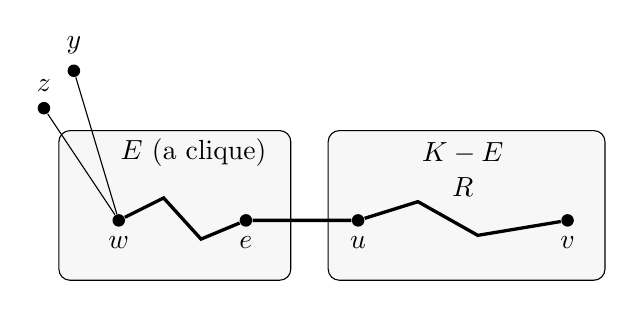
\begin{tikzpicture}[scale=.95,vertex/.style={circle,fill=black,inner sep=1.6pt}]
\draw[rounded corners,fill=black!3] (-.8,-.8) rectangle (2.3,1.2);
\node at (1,.9) {$E$ (a clique)};
\node[vertex,label=below:$w$] (w) at (0,0) {};
\node[vertex,label=below:$e$] (e) at (1.7,0) {};
\draw[very thick] (w) -- (.6,.3) -- (1.1,-.25) -- (e);
\draw[rounded corners,fill=black!3] (2.8,-.8) rectangle (6.5,1.2);
\node at (4.6,.9) {$K-E$};
\node[vertex,label=below:$u$] (u) at (3.2,0) {};
\node[vertex,label=below:$v$] (v) at (6,0) {};
\draw[very thick] (e) -- (u) -- (4,.25) -- (4.8,-.2) -- (v);
\node at (4.6,.45) {$R$};
\node[vertex,label=above:$y$] (y) at (-.6,2) {};
\node[vertex,label=above:$z$] (z) at (-1,1.5) {};
\draw (y)--(w) (z)--(w);
\end{tikzpicture}
\caption{The final construction in Lemma~\ref{clq:coloured-path}.
Every edge from $E$ to $K-E$ is incident with $u$.
A vertex $w\in E$ sees both $y$ and $z$. Choose a neighbour
$e\ne w$ of $u$ in $E$, traverse all of $E$ from $w$ to $e$,
and continue through $u$ along $R$. Prefixing the appropriate one of
$y,z$ to an exact initial segment gives the required cross-colour path.
The schematic shows this traversal; other edges are unspecified.}
\label{fig:clique-endpoints}
\end{figure}

\section{The cases of four- and five-cycles}
\label{sec:small}

We now rule out the minimal counterexample when $k=3$ or $k=4$.
Only the triangle guaranteed by Lemma~\ref{clq:triangle} is needed
from the preceding section. The argument examines the neighbors
outside a clique and uses the absence of the required exact cycle
to separate their neighborhoods.

\begin{proposition}\label{small:cases}
Let $k\in\{3,4\}$ and let $a$ be an integer with $2\le a\le k$.
There is no graph $G$ with
\[
  |V(G)|=ka+1,\qquad \alpha(G)\le a,
  \qquad G\text{ contains no }C_{k+1},
\]
such that $|N_G[I]|\ge k|I|+1$ for every nonempty independent set
$I\subseteq V(G)$.
\end{proposition}

\begin{proof}
Suppose such a graph exists. Applying the neighborhood bound to a
singleton gives $\delta(G)\ge k$. Lemma~\ref{clq:triangle} supplies
a triangle, and a clique of order $k+1$ would contain the forbidden
cycle, so $3\le\omega(G)\le k$.

For a clique $Q=\{q_1,\ldots,q_t\}$, let $F=G-Q$ and put
\[
  U_i=N_G(q_i)\cap V(F)\qquad(1\le i\le t).
\]
We will use this notation with different choices of $Q$, specifying
the choice each time. A path between two distinct vertices of $Q$
whose internal vertices lie in $F$ can be completed using edges of
$Q$. The exact numbers of internal vertices that are forbidden are
checked below.

\medskip
\noindent\textbf{The case $k=3$.}
Choose a triangle $Q=\{q_1,q_2,q_3\}$. Each $U_i$ is nonempty,
since $q_i$ has two neighbors inside $Q$ and degree at least three.
For distinct $i,j$, write $h$ for the remaining index. A common
vertex $u\in U_i\cap U_j$ would give the cycle
\[
  q_i,u,q_j,q_h,q_i
\]
of order four. If $u\in U_i$ and $v\in U_j$ were adjacent, then
\[
  q_i,u,v,q_j,q_i
\]
would be a cycle of order four. Thus the sets $U_1,U_2,U_3$ are
pairwise disjoint and pairwise anticomplete.

Choosing one vertex from each $U_i$ gives an independent set of
order three. Hence $a=3$. If any $U_i$ contained two nonadjacent
vertices, adjoining one vertex from each of the other two sets would
give an independent set of order four. Therefore each $U_i$ is a
clique. Moreover, $\{q_i\}\cup U_i$ is a clique and there is no
$K_4$, so
\[
  1\le |U_i|\le2.
\]
Since $|V(F)|=7$, the set
\[
  W=V(F)\setminus(U_1\cup U_2\cup U_3)
\]
is nonempty. Every vertex of $W$ has no neighbor in $Q$ by the
definition of the $U_i$.

Fix $w\in W$. If $w$ saw two distinct vertices $u,v\in U_i$, then
$w,u,q_i,v,w$ would be a $C_4$. Thus $w$ has at most one neighbor
in each $U_i$. On the other hand, if $w$ missed a vertex $u\in U_i$
and a vertex $v\in U_j$ for distinct $i,j$, then
$\{w,u,v,q_h\}$ would be an independent set of order four. Indeed,
$w$ misses $Q$, the two exterior sets are anticomplete, and $q_h$
has no neighbor in either of them. It follows that $w$ is adjacent
to every vertex of at least two of the $U_i$. These two sets must
therefore be singletons.

There are consequently at least two singleton sets among the three
$U_i$. If exactly two are singletons, the three sizes are $1,1,2$,
so $|W|=3$. Every vertex of $W$ sees the two singleton vertices,
say $u,v$. Distinct $w,w'\in W$ then give the cycle
$w,u,w',v,w$ of order four. If all three $U_i$ are singletons,
then $|W|=4$. Each $w\in W$ sees at least two of the three singleton
vertices. Choose one pair of such neighbors for each $w$. There are
only three pairs, so two vertices $w,w'$ choose the same pair
$\{u,v\}$, again giving $w,u,w',v,w$. This rules out $k=3$.

\medskip
\noindent\textbf{The case $k=4$ with a clique of order four.}
Suppose first that $Q=\{q_1,q_2,q_3,q_4\}$ is a clique. A path
between distinct $q_i,q_j$ with one, two, or three internal vertices
outside $Q$ can be completed to a $C_5$ by a path in $Q$ of length
three, two, or one, respectively. More explicitly, with $q_h,q_\ell$
the other clique vertices, the prohibited configurations yield
\[
\begin{gathered}
  q_i,u,q_j,q_h,q_\ell,q_i,\\
  q_i,u,v,q_j,q_h,q_i,\\
  q_i,u,z,v,q_j,q_i.
\end{gathered}
\]
In every row the exterior vertices are distinct and lie outside
$Q$, so the displayed cycle has exactly five vertices.

The sets $U_i$ are nonempty. Their closed neighborhoods in $F$ are
pairwise disjoint: an intersection of $N_F[U_i]$ and $N_F[U_j]$
would give vertices $u\in U_i$, $v\in U_j$ at distance at most two
in $F$, with $u=v$ allowed. A shortest such path, joined to $q_i$
and $q_j$, is one of the three prohibited configurations. In
particular, every vertex $u\in U_i$ has exactly one neighbor in
$Q$, so it has at least three neighbors in $F$. It follows that
\[
  |V(F)|\ge\sum_{i=1}^4|N_F[U_i]|\ge4\cdot4=16.
\]
But $|V(F)|=4a-3\le13$, a contradiction. We may therefore assume
that $\omega(G)=3$.

\medskip
\noindent\textbf{Triangles with disjoint exterior neighbor sets.}
For any triangle $Q=\{q_1,q_2,q_3\}$, every $U_i$ has size at
least two. A path between distinct triangle vertices with two or
three internal vertices outside $Q$ gives a $C_5$. In particular,
if distinct $u\in U_i$, $v\in U_j$ are adjacent, or are joined by
a two-edge path $u,z,v$ in $F$, the respective cycles are
\begin{equation}
  q_i,u,v,q_j,q_h,q_i
  \qquad\text{and}\qquad
  q_i,u,z,v,q_j,q_i,
  \label{small:five-cycles}
\end{equation}
where $h$ is the remaining triangle index.

Suppose for the moment that $U_1,U_2,U_3$ are disjoint. By
\eqref{small:five-cycles}, their closed neighborhoods in $F$ are
also pairwise disjoint. A maximum independent subset $J$ of $U_i$
has exactly one neighbor in $Q$, namely $q_i$. Thus the assumed
expansion bound gives
\begin{equation}
  |N_F[U_i]|\ge |N_F[J]|
  =|N_G[J]|-1\ge4\alpha(U_i).
  \label{small:one-neighbor-count}
\end{equation}
Here $|V(F)|=4a-2\le14$. If any $U_i$ had independence number at
least two, the three disjoint neighborhoods would together have
at least $8+4+4=16$ vertices. Hence every $U_i$ is a clique. Its
size is exactly two, because it has size at least two and adjoining
$q_i$ cannot produce a $K_4$.

If the exterior neighbor sets were disjoint for every triangle,
write $U_i=\{u_i,v_i\}$ and apply that assertion to the triangle
$T_i=\{q_i,u_i,v_i\}$. Each of $u_i,v_i$ has at least two neighbors
outside $T_i$, and the two sets of such neighbors are disjoint.
All of these vertices lie in $F-U_i$: the original disjointness
prevents $u_i$ or $v_i$ from seeing a vertex of $Q\setminus\{q_i\}$.
Consequently $|N_F[U_i]|\ge2+2+2=6$ for every $i$. The three
original closed neighborhoods are disjoint, so this would require
at least $18$ vertices in $F$, again impossible. Some triangle
therefore has overlapping exterior neighbor sets.

\medskip
\noindent\textbf{The necessary structure at an overlapping triangle.}
Take a triangle for which
$I=U_1\cap U_2\ne\varnothing$. No other pair of exterior sets
overlaps. Indeed, a vertex in all three sets would form a $K_4$
with $Q$. If $x\in U_1\cap U_2$ and
$y\in U_1\cap U_3$ are distinct, then
\[
  q_2,x,q_1,y,q_3,q_2
\]
is a $C_5$; if instead $y\in U_2\cap U_3$, use
$q_1,x,q_2,y,q_3,q_1$. Also $I$ is independent, since adjacent
vertices $x,y\in I$ would give the $K_4$ on $q_1,q_2,x,y$.

The four sets
\[
  I,\qquad A=U_1\setminus I,\qquad
  B=U_2\setminus I,\qquad D=U_3
\]
have pairwise disjoint closed neighborhoods in $F$. To check this
even for pairs involving $I$, choose distinct triangle neighbors
for vertices in the six possible pairs of classes as follows:
\[
\begin{array}{c|cccccc}
\text{classes}&(I,A)&(I,B)&(I,D)&(A,B)&(A,D)&(B,D)\\ \hline
\text{neighbors}&(q_2,q_1)&(q_1,q_2)&(q_1,q_3)&
                  (q_1,q_2)&(q_1,q_3)&(q_2,q_3).
\end{array}
\]
If two vertices from the indicated classes were adjacent or shared
a neighbor in $F$, the corresponding distinct triangle neighbors
would close one of the cycles in \eqref{small:five-cycles}. Since
the classes themselves are disjoint, their closed neighborhoods
are disjoint as claimed.

Write $r=|I|$. The set $I$ is independent and its only neighbors in
$Q$ are $q_1,q_2$. Hence
\begin{equation}
  |N_F[I]|=|N_G[I]|-2\ge4r-1.
  \label{small:overlap-count}
\end{equation}
Each nonempty one of $A,B,D$ has exactly one triangle neighbor,
so the argument of \eqref{small:one-neighbor-count} bounds the
size of its closed neighborhood below by four times its
independence number. These bounds may be added because the four
closed neighborhoods are disjoint.

If $r=1$, then both $A$ and $B$ are nonempty, since
$|U_1|,|U_2|\ge2$, and $D$ is nonempty as well. The four
neighborhoods would have total size at least
$3+4+4+4=15>14$. If $r\ge3$, the neighborhoods of $I$ and $D$
alone would have total size at least $11+4=15>14$. Thus $r=2$.
In this case the neighborhoods of $I$ and $D$ already contribute
at least $7+4=11$ vertices; a nonempty $A$ or $B$ would increase
the bound to $15$. Therefore
\begin{equation}
  |I|=2,\qquad U_1=U_2=I.
  \label{small:overlap-structure}
\end{equation}
Moreover, $\alpha(D)\ge2$ would give $7+8=15$ vertices, so $D$
is a clique. Its size is exactly two, by the degree bound and the
absence of a $K_4$.

This argument proves a necessary statement for \emph{every}
triangle with overlapping exterior neighbor sets: exactly one
pair overlaps, both sets in that pair equal an independent set
of size two, and the third exterior neighbor set is a clique of
size two. No condition on the exterior sets of other triangles
was used in proving this statement.

\medskip
\noindent\textbf{The final contradiction.}
Write $I=\{w,z\}$ and consider the triangle
$T=\{q_1,q_2,w\}$. By \eqref{small:overlap-structure}, the
exterior neighbor sets of its first two vertices are both
\[
  N_G(q_1)\setminus T=N_G(q_2)\setminus T=\{q_3,z\}.
\]
The necessary statement just proved therefore applies to $T$.
Its third vertex $w$ has exactly two neighbors outside $T$.
Neither $q_3$ nor $z$ is adjacent to $w$: adjacency to $q_3$
would give a $K_4$ with the original triangle, and $I$ is
independent. Thus the neighbors of $w$ outside $T$ are precisely
its neighbors in the original graph $F$, and $d_F(w)=2$.
The same reasoning applies to $z$. Consequently,
\[
  |N_F[I]|\le |I|+d_F(w)+d_F(z)=2+2+2=6,
\]
whereas \eqref{small:overlap-count} gives $|N_F[I]|\ge7$.
This contradiction completes the case $k=4$ and the proof.
\end{proof}

By Lemma~\ref{red:expansion}, the minimal counterexample satisfies
all the assumptions of Proposition~\ref{small:cases}. Hence we
may assume $k\ge5$ from now on.

\section{From size to independence}\label{sec:size}

We next show that a vertex set larger than both $k$ and twice the clique
number contains three independent vertices.  The argument uses only the
forbidden cycle and the clique bound.  We first prove two elementary facts
about graphs with independence number at most two.
The first is a special case of the Chv\'atal--Erd\H{o}s Hamiltonicity
theorem~\cite[Theorem~1]{ChvatalErdos1972}. The shortening argument in the
second appears in Radziszowski and Jin's proof of their pancyclicity
theorem~\cite[Theorem~2]{RadziszowskiJin1994}. We include both proofs.

\begin{lemma}\label{size:hamiltonian}
Every finite simple 2-connected graph $H$ with $\alpha(H)\le2$ contains a
cycle through all its vertices.
\end{lemma}

\begin{proof}
A 2-connected graph has minimum degree at least two and therefore contains
a cycle: all neighbors of an endpoint of a longest path lie on that path,
and two such neighbors give a cycle.  Choose a cycle $C$ of maximum order,
orient it, and write $a^+$ for the successor of $a\in V(C)$.

Suppose that a component $D$ of $H-V(C)$ exists.  Its set of neighbors on
$C$ contains at least two vertices.  Indeed, it is nonempty by
connectedness, and a unique such vertex would be a cutvertex of $H$.
If $a\in V(C)$ has a neighbor in $D$, then $a^+$ has none.  Otherwise a
path from $a$ to $a^+$ with nonempty interior in the connected graph $D$
could replace the edge $aa^+$, giving a longer cycle.  This path exists
even if $a$ and $a^+$ have the same neighbor in $D$.

Choose distinct vertices $a,b\in V(C)$ with neighbors in $D$, and a path
$P$ from $a$ to $b$ with nonempty interior in $D$.  The vertices $a^+,b^+$
are distinct, neither equals $a$ or $b$, and both have no neighbor in $D$.
If $a^+b^+$ were an edge, we could traverse $P$ from $a$ to $b$, follow
$C$ backwards from $b$ to $a^+$, use $a^+b^+$, and follow $C$ forwards
from $b^+$ to $a$.  Deleting $aa^+$ and $bb^+$ from $C$ leaves exactly
the two cycle segments used here.  Hence this would be a cycle containing
every vertex of $C$ and at least one additional vertex, a contradiction.
Thus $a^+$ and $b^+$ are nonadjacent.  Together with any vertex of $D$,
they form an independent triple, also a contradiction.  Therefore $C$
is spanning.
\end{proof}

\begin{lemma}\label{size:shortening}
Let $H$ be a finite simple graph on $r\ge7$ vertices with
$\alpha(H)\le2$.  If $H$ has a Hamiltonian cycle, then it has a cycle
on exactly $r-1$ vertices.
\end{lemma}

\begin{proof}
Label the vertices around a Hamiltonian cycle by $0,1,\ldots,r-1$, with
indices interpreted modulo $r$.  If some edge joins $i$ to $i+2$, it
bypasses the vertex $i+1$ and gives the required cycle.  Suppose there
is no such edge.  In each triple $i,i+2,i+4$, the pairs $i(i+2)$ and
$(i+2)(i+4)$ are nonedges.  Since the triple is not independent,
$i(i+4)$ is an edge.  All cyclic step-four edges are therefore present.

Consider the cyclic sequence
\begin{equation}\label{size:shortening-cycle}
 1,2,\ldots,r-6,\quad r-2,r-1,\quad r-5,r-4,r-3,\quad1.
\end{equation}
Before closing, its three blocks partition the vertices $1,\ldots,r-1$.
Consecutive vertices within a block are adjacent on the original cycle.
The three edges joining the blocks and closing the sequence are
\[
 (r-6)(r-2),\qquad (r-1)(r-5),\qquad (r-3)1;
\]
their cyclic differences are $4,-4,4$, respectively.  Thus
\eqref{size:shortening-cycle} is a cycle of order $r-1$.
When $r=7$, the first block is the singleton $1$, and the sequence is
explicitly $1,5,6,2,3,4,1$, so the same construction applies.
\end{proof}

\begin{lemma}[Size test]\label{size:test}
Let $k\ge5$ and $t\ge1$ be integers.  Let $G$ be a finite simple graph
with no cycle on exactly $k+1$ vertices and with clique number at most
$t$.  For every $Y\subseteq V(G)$,
\[
 |Y|>\max\{k,2t\}\quad\Longrightarrow\quad\alpha(G[Y])\ge3.
\]
\end{lemma}

\begin{proof}
Suppose that $H=G[Y]$ has $\alpha(H)\le2$ and order
$n>\max\{k,2t\}$.  If $H$ is disconnected, it has exactly two
components, each a clique.  Indeed, three components give an independent
triple, as does a nonadjacent pair in one component together with a vertex
of another.  The two cliques have at most $t$ vertices each, contrary to
$n>2t$.

If $H$ has a cutvertex $v$, the same argument shows that $H-v$ has
exactly two components $A,B$, both cliques of order at most $t$.
The inequalities
\[
 |A|+|B|+1=n>2t,\qquad |A|,|B|\le t
\]
force $|A|=|B|=t$.  The vertex $v$ must be adjacent to all of one
component: a nonneighbor in each would form an independent triple with
$v$.  That component together with $v$ is a clique of order $t+1$,
again a contradiction.

Consequently $H$ is 2-connected and has a Hamiltonian cycle by
Lemma~\ref{size:hamiltonian}.  Its order is $n\ge k+1$.  If a current
cycle has order $r>k+1$, the graph induced by its vertices is Hamiltonian,
has independence number at most two, and satisfies $r\ge k+2\ge7$.
Lemma~\ref{size:shortening} therefore produces a cycle of order $r-1$.
Repeated shortening reaches exactly $k+1$, contradicting the hypothesis
on $G$.
\end{proof}

\section{Optimal path systems}\label{sec:paths}

We now assume $k\geq5$ and work in the graph $G$ from the
minimal-counterexample reduction. Thus $G$ has no cycle of order $k+1$,
$\delta(G)\geq k$, $\alpha(G)\leq k$, and the independent-set expansion
of Lemma~\ref{red:expansion} holds. Fix a maximum clique $Q$, and write
\[
 t=|Q|,\qquad h=k+1-t.
\]
By Theorem~\ref{clq:bound},
$\max(3,\lfloor k/2\rfloor)\leq t\leq k$, so $h\geq1$.
Our first objective is to encode paths through vertices outside $Q$ in a
way that allows us to close them into a cycle of exactly the forbidden
order. We then choose an optimal encoding and relate short paths outside
its vertex set to separated sets of vertices.

\subsection{Paths joining clique vertices}

A \emph{path system on $Q$} is a collection $\mathcal R$ of simple paths
with the following properties. Each path has two distinct endpoints in
$Q$ and a nonempty interior contained in $V(G)\setminus Q$. The interiors
of different paths are disjoint. Represent each path by the edge joining
its endpoints in an auxiliary graph with vertex set $Q$. These represented
edges must be distinct and must form a linear forest: every component is
a path, including isolated vertices. We call these components
\emph{chains}. In particular, every unused clique vertex is a singleton
chain; it does not represent a path with empty interior.

The \emph{amount} of an assigned path is its number of internal vertices.
For a system $\mathcal R$, let $q(\mathcal R)$ be the sum of its amounts,
let $e(\mathcal R)$ be its number of assigned paths, and let
$v(\mathcal R)$ be the number of clique vertices incident with its
represented edges. Thus singleton chains contribute neither to the amount
nor to the incident-vertex count. The empty collection is allowed.

\begin{lemma}[Closing a path system]\label{path:interval}
Let $G$ be a finite simple graph with no cycle of order $k+1$, and let
$Q$ be a clique of size $t$, where $3\leq t\leq k$.
Put $h=k+1-t$. No path system on $Q$, of total amount $q$ and with $v$
incident clique vertices, satisfies
\begin{equation}\label{path:forbidden-interval}
 h\leq q\leq k+1-v.
\end{equation}
\end{lemma}

\begin{proof}
Suppose such a system exists. The integer
\[
 u=k+1-q-v
\]
satisfies $0\leq u\leq t-v$: the first inequality follows from the upper
bound on $q$, and the second from $q\geq h$. Choose exactly $u$ of the
clique vertices not incident with represented edges.

Expand each nontrivial chain by replacing its represented edges with
their assigned paths. Each expansion is a simple path, and different
expansions are vertex-disjoint. Indeed, their clique vertices belong to
different forest components, and all assigned interiors are disjoint and
lie outside $Q$. Adjoin the $u$ chosen unused clique vertices as singleton
paths. These paths together contain exactly
\[
 q+v+u=k+1
\]
vertices, and all their endpoints belong to $Q$.

There is at least one nontrivial expanded chain, since $q\geq h\geq1$.
If there is only one path in the resulting list, it has at least three
vertices: it contains an assigned path with nonempty interior. The clique
edge between its distinct endpoints closes it into a simple cycle. If
there are two or more paths, order and orient them arbitrarily, join each
path's last endpoint to the next path's first endpoint by a clique edge,
and close the last to the first. This again gives a simple cycle. In the
case of two paths with one singleton, the two joining edges use the two
distinct endpoints of the nontrivial path; thus they are distinct. The
case of two singleton paths cannot occur. All remaining cases follow
directly from vertex-disjointness. The resulting cycle has order $k+1$,
a contradiction.
\end{proof}

Choose a path system $\mathcal P$ of maximum total amount $L$ subject to
$L<h$. Among systems with this amount, choose one with the minimum number
$e$ of assigned paths. This choice exists: the empty system has amount
zero, and $G$ is finite. Write
\begin{equation}\label{path:system-vertices}
 S=Q\cup\bigcup_{P\in\mathcal P}\bigl(V(P)\setminus Q\bigr),
 \qquad F=G-S.
\end{equation}
Since the amounts are positive integers and the interiors are disjoint,
\begin{equation}\label{path:budget}
 0\leq e\leq L\leq h-1=k-t,
 \qquad |S|=t+L\leq k.
\end{equation}
In particular, $L=0$ forces $e=0$; this includes the case $t=k$.

The choice of $\mathcal P$ and Lemma~\ref{path:interval} give a single
criterion that we will apply to modified systems.

\begin{lemma}[Optimality criterion]\label{path:optimality}
Let $\mathcal R$ be any path system on $Q$, with total amount $A$, with
$e'$ assigned paths, and with $v'$ incident clique vertices. Then
\begin{equation}\label{path:optimality-interval}
 L+\mathbf 1_{\{e'\geq e\}}\leq A\leq k+1-v'
\end{equation}
is impossible, where the indicator is one when $e'\geq e$ and zero
otherwise.
\end{lemma}

\begin{proof}
If $A\geq h$, Lemma~\ref{path:interval} applies. If $A<h$ and $e'\geq e$,
the lower bound gives $A\geq L+1$, contrary to the maximality of $L$.
If $A<h$ and $e'<e$, that lower bound gives $A\geq L$. Strict inequality
again contradicts maximality, and equality contradicts the choice of $e$.
\end{proof}

\begin{lemma}\label{path:exterior}
Every vertex of $S$ has at least $k+1-|S|\geq1$ neighbors in $F$.
\end{lemma}

\begin{proof}
A vertex of $S$ has at most $|S|-1$ neighbors in $S$ and has degree at
least $k$. Now use~\eqref{path:budget}.
\end{proof}

\subsection{Outside paths and separated balls}

The next definitions apply to any set $X\subseteq V(G)$; later $X$ will
be $S$ or a set obtained by adding vertices to $S$. For distinct
$x,y\in X$, an \emph{outside path relative to $X$ with parameter $d$}
is a simple $x$--$y$ path with exactly $d$ internal vertices, all in
$V(G)\setminus X$. Its length is $d+1$. We allow $d=0$, which means
the edge $xy$.

For $x\in X$, define subsets of $V(G)\setminus X$ by
\begin{equation}\label{path:balls}
 B_0(x;X)=N_G(x)\setminus X,
 \qquad
 B_{r+1}(x;X)=N_{G-X}[B_r(x;X)]\quad(r\geq0).
\end{equation}
Thus $B_r(x;X)$ consists of the vertices at distance at most $r$ in
$G-X$ from the outside-neighbor set $B_0(x;X)$. Every vertex of this
ball is joined to $x$ by a path of at most $r+1$ edges whose remaining
vertices lie outside $X$. The balls are nested and may be empty.

\begin{lemma}[Separation by forbidden outside paths]\label{path:separation}
Let $X\subseteq V(G)$ and let $x,y\in X$ be distinct.
\begin{enumerate}
\item For integers $r,s\geq0$, if no outside $x$--$y$ path relative to
$X$ has parameter $d$ with $1\leq d\leq r+s+2$, then
$B_r(x;X)$ and $B_s(y;X)$ are disjoint and anticomplete.
\item For an integer $r\geq1$, if no such path has parameter
$1\leq d\leq r$, then $y$ has no neighbor in $B_{r-1}(x;X)$.
\end{enumerate}
\end{lemma}

\begin{proof}
If the two balls in the first assertion meet, concatenate their paths
from $x$ and $y$ to a common vertex. This gives an $x$--$y$ walk of at
most $r+s+2$ edges, all of whose internal vertices lie outside $X$.
Deleting repeated portions produces a simple outside path with at most
$r+s+1$ internal vertices. If instead an edge joins the two balls, use
that edge between the two paths. The resulting walk has at most
$r+s+3$ edges and yields an outside path with at most $r+s+2$ internal
vertices. In both cases the parameter is at least one, since the walk
has no direct step from $x$ to $y$. Each case contradicts the hypothesis.

For the second assertion, a vertex of $B_{r-1}(x;X)$ has a path from
$x$ of at most $r$ edges with all subsequent vertices outside $X$.
If that vertex were adjacent to $y$, appending the edge to $y$ would
give an outside path with between one and $r$ internal vertices.
\end{proof}

When choosing separated sets, we also allow the singleton $\{x\}$ as
an option with \emph{radius label $-1$}. This is a separate convention;
it is not an additional step of the recursion~\eqref{path:balls}.
An option with radius $r\geq0$ means the ball $B_r(x;X)$.

\begin{corollary}[Singleton and ball compatibility]\label{path:singleton}
Consider two options based at distinct vertices $x,y\in X$, with
integer radius labels $r,s\geq-1$. If $r=s=-1$, the two options are disjoint
and anticomplete whenever $xy\notin E(G)$. Otherwise, they are disjoint
and anticomplete whenever all outside $x$--$y$ paths relative to $X$
with parameters
\[
 1\leq d\leq r+s+2
\]
are forbidden.
\end{corollary}

\begin{proof}
The case of two singletons is immediate, and the case $r,s\geq0$ is
Lemma~\ref{path:separation}. It remains to consider $r=-1$ and $s\geq0$,
after interchanging the options if necessary. The singleton $\{x\}$
and the ball $B_s(y;X)$ are disjoint because they lie in $X$ and
$V(G)\setminus X$, respectively. An edge between them would give an
outside $x$--$y$ path with between one and $s+1=r+s+2$ internal vertices,
contrary to the hypothesis.
\end{proof}

Pairwise separated options allow independent sets chosen in them to be
combined. In particular, if their individual independence numbers are
at least $u_1,\ldots,u_j$, then $G$ has an independent set of size at
least $u_1+\cdots+u_j$. We will use this observation to turn the path
restrictions imposed by optimality into a contradiction to
$\alpha(G)\leq k$.

\section{Short paths between representatives}\label{sec:growth}

We retain the optimal path system $\mathcal P$ and the notation
$Q,t,h,L,e,S,F$ from Section~\ref{sec:paths}, and assume throughout
this section that $t\ge 9$.
We shall choose one vertex of $S$ for each vertex of $Q$ so that an
outside path between two chosen vertices can be inserted into the
system without losing any of its old interior vertices.  Neighborhood
expansion will then force such an outside path with at most six
internal vertices.

Orient each chain of the forest represented by $\mathcal P$.
For each \emph{target} $q\in Q$, define its \emph{representative}
$\rho(q)\in S$ as follows.  If $q$ is the first vertex of its chain,
including a singleton chain, set $\rho(q)=q$.  Otherwise its incoming
path, read in the chosen orientation, has the form
\[
 p,z_1,z_2,\ldots,z_a,q,\qquad a\ge 1;
\]
set $\rho(q)=z_1$, the first interior vertex after the predecessor $p$.
The segment from $\rho(q)$ to $q$ therefore contains all $a$ interior
vertices of the incoming path.  The representatives are distinct,
since different incoming paths have disjoint interiors and only
chain starts are represented by clique vertices.  Write
$R=\{\rho(q):q\in Q\}$, so $|R|=t$.

\begin{lemma}[Replacing incoming paths]\label{grow:replacement}
Fix an orientation of the chains and distinct targets $q,q'\in Q$.
Suppose an outside path relative to $S$ joins $\rho(q)$ to $\rho(q')$
and has $d\ge 1$ internal vertices.  Let $r\in\{0,1,2\}$ be the number
of these two targets that have an incoming path.
Deleting those $r$ paths from $\mathcal P$ and inserting one new path
from $q$ to $q'$ gives a valid path system with total amount $L+d$
and $e+1-r$ paths.  It retains all the interior vertices of
$\mathcal P$.
\end{lemma}

\begin{proof}
At each target with an incoming path, retain its segment from the
representative to the target.  At a chain start the corresponding
segment consists only of the target.  Concatenate the reverse of the
segment at $q$, the given outside path, and the segment at $q'$.
Figure~\ref{fig:representatives} illustrates the construction with two
incoming paths.
The two retained segments have disjoint interiors, and the outside
path has its interior in $F=G-S$, so the resulting path is simple.
In particular, a retained segment contains no clique vertex except
its own target.  This remains true when the two targets are
consecutive on one chain.

After deleting the incoming paths, each target has degree at most
one in the represented forest, and the targets lie in different
components.  If they belonged to different chains, this is immediate.
If they belonged to the same chain, deleting the incoming edge at
the later target separates them.  The new edge between the targets
thus creates neither a cycle nor a vertex of degree greater than
two.  It gives a valid linear forest.

If the deleted paths have total amount $A$, their retained segments
contribute exactly $A$ interior vertices to the new path.  Its amount
is therefore $A+d$, while the unchanged paths contribute $L-A$.
The total is $L+d$, and the number of paths is $e-r+1$.
\end{proof}

\begin{lemma}[One-vertex detours]\label{grow:one}
For every orientation of the chains, no outside path relative to $S$
with one internal vertex joins two distinct representatives.
Nor can such a path join consecutive vertices of any path of
$\mathcal P$.
\end{lemma}

\begin{proof}
The first type of path would give a system of amount $L+1$ by
Lemma~\ref{grow:replacement}.  For the second type, replace the step
between the consecutive vertices by the proposed two-edge path.
This keeps the represented forest and every old interior vertex,
again increasing the amount to $L+1$.

Since $L<h$, either $L+1<h$, contrary to maximality of $L$, or
$L+1=h$.  In the latter case the new system has at most $t$ incident
clique vertices, and hence lies in the forbidden interval of
Lemma~\ref{path:interval}.
\end{proof}

We next translate these exclusions into growth of the balls defined
in Section~\ref{sec:paths}.  Fix an orientation and a representative
$x\in R$.  An outside neighbor $u\in B_0(x;S)$ exists because
$|S|\le k$ and $\delta(G)\ge k$.  By Lemma~\ref{grow:one}, $u$ misses
the other $t-1$ representatives.  Since its closed neighborhood in
$F$ lies in $B_1(x;S)$, we obtain
\begin{equation}\label{grow:degree}
 |B_1(x;S)|
 \ge 1+\deg_F(u)
 \ge 1+k-\bigl(|S|-(t-1)\bigr)
 =k-|S|+t.
\end{equation}
Moreover, if some $y\in S\setminus R$ is missed by every vertex of
$B_0(x;S)$, the same count improves the right-hand side by one.
Only the one-vertex exclusions are needed for this degree estimate.

\begin{lemma}[Independence in the second ball]\label{grow:weights}
Fix an orientation and $x\in R$.  Suppose no outside path relative
to $S$ with one or two internal vertices joins $x$ to any other
representative.  Then
\[
 \alpha\bigl(B_2(x;S)\bigr)\ge 2.
\]
If, in addition, $B_1(x;S)$ is not a clique and $t<k$, then
$\alpha(B_2(x;S))\ge 3$.
\end{lemma}

\begin{proof}
Every vertex of $B_1(x;S)$ misses $R\setminus\{x\}$: an adjacency
to another representative would give an outside path with one or
two internal vertices.

Suppose first that $B_2(x;S)$ were a clique.  It contains
$B_1(x;S)$, whose order is at least $k-|S|+t\ge t$ by
\eqref{grow:degree}.  Since the maximum clique size is $t$, this forces
\[
 B_1(x;S)=B_2(x;S),\qquad |B_1(x;S)|=t,\qquad |S|=k.
\]
Each vertex $z$ of this ball has at most $t-1$ neighbors in $F$,
because all those neighbors lie in $B_2(x;S)$.  It also has at most
$k-t+1$ neighbors in $S$, since it misses the other representatives.
As $\deg_G(z)\ge k$, both bounds are attained.  In particular every
such $z$ is adjacent to $x$.  The ball together with $x$ is then a
clique of order $t+1$, a contradiction.  Thus $B_2(x;S)$ is not a
clique and has an independent pair.

Now suppose that $B_1(x;S)$ contains an independent pair $I$.
Its closed neighborhood in $F$ lies in $B_2(x;S)$, and its
neighborhood in $S$ avoids $R\setminus\{x\}$.  The expansion bound
of Lemma~\ref{red:expansion} gives
\begin{equation}\label{grow:pair-expansion}
 |B_2(x;S)|
 \ge 2k+1-\bigl(|S|-(t-1)\bigr)
 =2k-|S|+t
 \ge k+t.
\end{equation}
When $t<k$, this is greater than $\max(k,2t)$, so
Lemma~\ref{size:test} gives an independent triple.
\end{proof}

The independent pairs in the second balls may already give a
contradiction.  When they do not, the only remaining obstruction to
obtaining independent triples is a first ball that is a clique of
order $t$ with $|S|=k$.  In that case, the structure of the path
system will supply an additional excluded neighbor for at least two
representatives.

\begin{lemma}[A short outside path]\label{grow:short}
Suppose $t\ge 9$.  For every fixed orientation of the chains of
$\mathcal P$, two distinct representatives are joined by an outside
path relative to $S$ with $1\le d\le 6$ internal vertices.
By Lemma~\ref{grow:one}, such a path in fact has $2\le d\le 6$.
\end{lemma}

\begin{proof}
Fix an orientation and suppose that no such path exists.
Lemma~\ref{path:separation} makes the $t$ balls
$B_2(x;S)$, $x\in R$, pairwise disjoint and anticomplete.
Each has an independent pair by Lemma~\ref{grow:weights}, so together
they give an independent set of order at least $2t$.
If $2t>k$, this contradicts $\alpha(G)\le k$; this also settles the
case $t=k$ without using the independent-triple conclusion.

We may therefore assume $2t\le k$.  The bound
$\lfloor k/2\rfloor\le t$ from Theorem~\ref{clq:bound} now gives
\begin{equation}\label{grow:parity}
 k\in\{2t,2t+1\}.
\end{equation}
In particular $t<k$, and it suffices to find two representatives
whose first balls are not cliques.  Lemma~\ref{grow:weights} would
then give a combined independent set of order at least
$2t+2>k$.

If $|S|<k$, equation~\eqref{grow:degree} gives
$|B_1(x;S)|>t$ at every representative, so any two suffice.
It remains to consider $|S|=k$.  In this case
$L=k-t>0$, and hence $e\ge 1$.

Suppose first that $e\ge 2$.  At least two representatives are
interior vertices of paths of $\mathcal P$.  For each such
representative $x$, let $y$ be the next vertex toward its target.
This vertex is not in $R$: it is either a later interior vertex of
the same path, or, when the amount is one, the target itself, which
is not a chain start.  By the consecutive-vertex assertion of
Lemma~\ref{grow:one}, every outside neighbor of $x$ misses $y$.
The improved degree count following \eqref{grow:degree} yields
\[
 |B_1(x;S)|\ge k-|S|+t+1=t+1.
\]
Thus the two chosen first balls are not cliques.

Finally suppose that $e=1$.  The represented forest has one
nonsingleton chain, consisting of a single edge, and $t-2\ge 7$
singleton chains.  Let $x$ be the representative of any singleton
chain.  Reverse the nonsingleton chain, leaving every other
orientation fixed, and let $y$ be its new starting clique vertex.
The vertex $y$ was not in the original representative set $R$,
whereas $x$ is a representative in both orientations.
Lemma~\ref{grow:one}, applied to the reversed orientation, shows that
every outside neighbor of $x$ misses $y$.  Consequently
$|B_1(x;S)|\ge t+1$ once again.  Choosing two singleton
representatives gives the two required noncliques and the final
contradiction.  The reversed orientation was used only for the
unconditional one-vertex exclusion; the assumed absence of paths
with up to six internal vertices concerned the original orientation
alone.
\end{proof}

\begin{figure}[htbp]
\centering
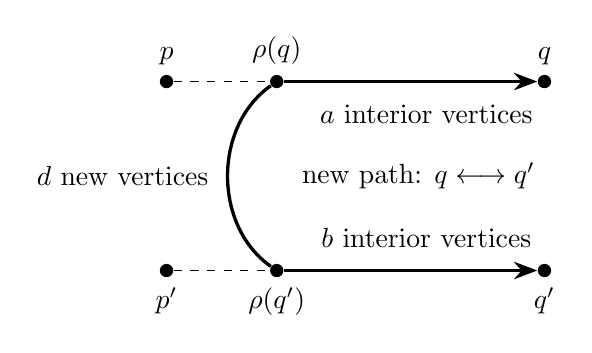
\begin{tikzpicture}[vertex/.style={circle,fill=black,inner sep=1.7pt},>=Stealth]
\node[vertex,label=above:$p$] (p) at (0,1.2) {};
\node[vertex,label=above:$\rho(q)$] (r) at (1.4,1.2) {};
\node[vertex,label=above:$q$] (q) at (4.8,1.2) {};
\node[vertex,label=below:$p'$] (pp) at (0,-1.2) {};
\node[vertex,label=below:$\rho(q')$] (rr) at (1.4,-1.2) {};
\node[vertex,label=below:$q'$] (qq) at (4.8,-1.2) {};
\draw[dashed] (p)--(r) (pp)--(rr);
\draw[very thick,->] (r)--(q);
\draw[very thick,->] (rr)--(qq);
\draw[very thick] (r) to[bend right=55] node[left,xshift=-3pt] {$d$ new vertices} (rr);
\node at (3.3,.78) {$a$ interior vertices};
\node at (3.3,-.78) {$b$ interior vertices};
\node at (3.2,0) {new path: $q\longleftrightarrow q'$};
\end{tikzpicture}
\caption{Representative replacement when both targets have incoming
paths. Each representative is the \emph{first} interior vertex on its
incoming path. Deleting the initial edge of each incoming path leaves its
full representative-to-target segment available. The new
path has amount $a+b+d$, so the entire system has amount $L+d$.
Lemma~\ref{grow:replacement} also treats a target at a chain start and
two targets on the same original chain. Dashed initial steps are not
used by the new path.}
\label{fig:representatives}
\end{figure}

\section{Excluding large cliques}\label{sec:terminal}

We retain the notation of Section~\ref{sec:paths} and assume \(t\ge9\).
Our goal is to obtain more than \(k\) independent vertices by combining
independent sets in separated balls.  Lemma~\ref{grow:short} supplies a short
outside path between representatives.  We first show that such a path forces
the optimal system \(\mathcal P\) into one of three configurations.
By Theorem~\ref{clq:bound},
\[
 t\le k\le2t+1,\qquad h=k+1-t,\qquad L\le k-t\le t+1.
\]

\subsection{A restriction on small increases in amount}

The next lemma applies to any valid replacement system, not only to the
construction between representatives.

\begin{lemma}\label{terminal:increment}
Let \(t\ge9\), and let \(\mathcal R\) be a valid path system consisting of some
paths of \(\mathcal P\) and one new path.  Suppose that its total amount is
\(L+d\), where \(1\le d\le6\).  Then
\[
 L=h-1=k-t.
\]
Moreover, \(\mathcal R\) contains all \(e\) paths of \(\mathcal P\), its new
path has amount \(d\), and every old path has amount at least \(d\).
In particular, a construction of this kind that removes an old path is
impossible.
\end{lemma}

\begin{proof}
If \(L+d<h\), then \(\mathcal R\) contradicts the maximality of \(L\).
Otherwise choose an inclusion-minimal subcollection of \(\mathcal R\) with
amount at least \(h\).  Write its amount as \(h+j\), its number of paths as
\(r\), and its number of incident clique vertices as \(w\).
The subcollection contains the new path, since the old paths have total
amount \(L<h\).  Also
\[
 0\le j\le5,
\]
because \(h+j\le L+d\le h+5\).
Lemma~\ref{path:interval} gives
\[
 h+j>k+1-w,\qquad\text{or equivalently}\qquad w>t-j.
\]
Since \(w\le t\), this also excludes \(j=0\).  Thus
\begin{equation}\label{terminal:minimal}
 1\le j\le5,\qquad 2r\ge w\ge t-j+1.
\end{equation}

Deleting any selected path lowers the amount below \(h\); consequently
every selected amount is at least \(j+1\).
Suppose that all were at least \(j+2\).
Exactly \(r-1\) of the selected paths are old, so
\[
 (r-1)(j+2)\le L\le k-t.
\]
Together with \eqref{terminal:minimal}, this implies
\[
 (t-j-1)(j+2)\le2(k-t)\le2t+2.
\]
The left side is a concave function of \(j\) on \([1,5]\).
Its endpoint values are \(3(t-2)\) and \(7(t-6)\), whose differences from
\(2t+2\) are respectively \(t-8\) and \(5t-44\).
Both are positive for \(t\ge9\), a contradiction.

Some selected path therefore has amount exactly \(j+1\).
Deleting it, whether it is old or new, leaves a valid system of amount
\(h-1\).  Maximality gives \(L=h-1\).
The minimum-path tie-break in the choice of \(\mathcal P\) now gives
\(r-1\ge e\).
On the other hand, \(\mathcal R\) has at most \(e+1\) paths, so \(r\le e+1\).
Hence \(r=e+1\): the selected subcollection is all of \(\mathcal R\), and
all old paths occur in it.
Comparing its two expressions for the total amount gives
\[
 h+j=L+d=h-1+d,\qquad j=d-1.
\]
Thus every selected amount is at least \(j+1=d\), and, since all old paths
remain, the new path has amount exactly \(d\).
\end{proof}

\subsection{The three possible configurations}

Call a vertex of \(Q\) \emph{missing} if it is not incident to any path of
\(\mathcal P\).  Thus the missing vertices are precisely the singleton
chains of its represented forest.  Let \(v\) denote the number of incident
vertices, so there are \(t-v\) missing vertices.

\begin{lemma}\label{terminal:classification}
Suppose that, for some orientation of the chains, an outside path with
parameter \(d\in\{1,\ldots,6\}\) joins two representatives.
Then \(L=k-t\), and exactly one of the following alternatives holds:
\begin{enumerate}
 \item\label{terminal:two}
 \(d=2\), \(v\ge t-2\), and every old amount is at least two;
 \item\label{terminal:three}
 \(d=3\), \(t\in\{9,11\}\), \(e=(t-3)/2\), and \(v=t-3\);
 the old paths represent a matching and have amounts at least three;
 \item\label{terminal:five}
 \(d=5\), \(t=9\), \(k=19\), \(e=2\), and \(v=4\);
 the old paths represent a matching and both have amount five.
\end{enumerate}
In every alternative, the two targets must be starting vertices in their
oriented chains.  In Alternative~\ref{terminal:two} their union must contain
all missing vertices.  In Alternatives~\ref{terminal:three}
and~\ref{terminal:five} both targets must be missing.

Once one of these alternatives holds, its parameter and endpoint
restrictions apply to every outside path with parameter between one and six
between representatives, in every orientation.
\end{lemma}

\begin{proof}
Lemma~\ref{grow:replacement} constructs a valid system of amount \(L+d\),
consisting of unchanged old paths and one new path.
Lemma~\ref{terminal:increment} shows that no old path was removed.
The two targets must therefore be starting vertices, and every old amount
is at least \(d\).
The proof of Lemma~\ref{terminal:increment} also gives \(j=d-1\ge1\), so
\(d\ge2\).

Let \(a\in\{0,1,2\}\) be the number of missing targets among these two
vertices.  The new system has exactly \(v+a\) incident vertices.
Its amount is \(h+d-1\); hence Lemma~\ref{path:interval} gives
\begin{equation}\label{terminal:incident}
 v+a\ge t-d+2.
\end{equation}
In particular, \(v\ge t-d\).  Since \(v\le2e\) and every old amount is at
least \(d\), we obtain
\begin{equation}\label{terminal:arithmetic}
 2\le d\le6,\qquad
 d\left\lceil\frac{t-d}{2}\right\rceil
 \le de\le L=k-t\le t+1.
\end{equation}

For \(d=2\), this gives \(v\ge t-2\).
Equation~\eqref{terminal:incident} says that \(v+a\ge t\), so the two targets
must cover all \(t-v\) missing vertices.

For \(d=3\), dropping the ceiling in \eqref{terminal:arithmetic} gives
\(3(t-3)\le2(t+1)\), and hence \(t\le11\).
At \(t=10\), the exact bound fails because
\(3\lceil7/2\rceil=12>11\).
At \(t=9\) it forces \(e=3\), and at \(t=11\) it forces \(e=4\).
In each case
\[
 t-3\le v\le2e=t-3.
\]
Thus \(v=2e=t-3\), so no two old edges share a clique vertex.
Equation~\eqref{terminal:incident} then forces \(a=2\).

For \(d=4\), the weaker bound \(4(t-4)\le2(t+1)\) gives \(t\le9\);
but at \(t=9\) the exact bound fails:
\(4\lceil5/2\rceil=12>10\).
For \(d=5\), the weaker bound gives \(3t\le27\), hence \(t=9\).
Now \(2\le e\le2\) and \(4\le v\le2e=4\).
Moreover,
\[
 10=5e\le L\le t+1=10,
\]
so \(L=10\), \(k=19\), and both amounts are five.
Again \eqref{terminal:incident} forces \(a=2\).
Finally, for \(d=6\), the weaker bound gives \(4t\le38\), hence \(t=9\);
there \(6\lceil3/2\rceil=12>10\), which is impossible.

The three surviving alternatives are mutually exclusive properties of
the fixed old system: they require respectively
\[
 v\ge t-2,\qquad v=t-3,\qquad t=9,\ v=t-5.
\]
The argument applies to every orientation and every pair admitting a
path with parameter between one and six.  Thus, once the old system lies in
one alternative, any such path in any orientation must obey the corresponding
parameter and endpoint restrictions.
\end{proof}

\subsection{Independent sets in balls}

We next obtain bounds that apply to each representative individually.
When choosing several balls later, we will check their pairwise separation
separately.

\begin{lemma}\label{terminal:weights}
Under any alternative of Lemma~\ref{terminal:classification}, there are at
least two nonsingleton chains.
For every vertex \(x\) that is a representative in some orientation,
\[
 |B_1(x;S)|\ge t+1,\qquad \alpha(B_1(x;S))\ge2.
\]
If \(k\ge2t\), then also \(\alpha(B_2(x;S))\ge3\).
\end{lemma}

\begin{proof}
The matching in Alternative~\ref{terminal:three} has three or four edges,
and that in Alternative~\ref{terminal:five} has two.
In Alternative~\ref{terminal:two}, if there were only one nonsingleton
chain, then
\[
 v=e+1\le\left\lfloor\frac{t+1}{2}\right\rfloor+1<t-2,
\]
contrary to \(v\ge t-2\).
Here \(2e\le L\le t+1\) was used.
There cannot be no nonsingleton chain, since \(v\ge t-2>0\).

Fix an orientation in which \(x\) is a representative.
Choose a nonsingleton chain other than the chain containing its target,
and reverse only that chain.  Its old terminal clique vertex becomes a
representative, although it was not one of the original representatives;
meanwhile \(x\) remains a representative.
By Lemma~\ref{grow:one}, every vertex of \(B_0(x;S)\) is nonadjacent to the
other \(t-1\) original representatives and to this additional clique vertex.

Lemma~\ref{terminal:classification} gives \(|S|=t+L=k\).
The set \(B_0(x;S)\) is nonempty, because \(\delta(G)\ge k\) and
\(|S|\le k\).  For \(z\in B_0(x;S)\), its closed neighborhood has size at
least \(k+1\), meets \(S\) in at most \(|S|-t\) vertices, and is contained
in \(S\cup B_1(x;S)\).  Therefore
\[
 |B_1(x;S)|\ge k+1-(|S|-t)=t+1.
\]
Since \(t\) is the maximum clique size, this ball contains an independent
pair \(I\).  The expansion inequality \eqref{red:expansion-bound} and the
containment \(N_G[I]\subseteq S\cup B_2(x;S)\) give
\[
 |B_2(x;S)|\ge2k+1-|S|=k+1.
\]
If \(k\ge2t\), this exceeds \(\max(k,2t)\), so
Lemma~\ref{size:test} supplies an independent triple.
\end{proof}

\subsection{The final packings}

\begin{proposition}\label{terminal:contradiction}
There is no counterexample \(G\) with maximum clique size \(t\ge9\).
\end{proposition}

\begin{proof}
By Lemma~\ref{grow:short}, some pair of representatives admits an outside
path with parameter between one and six.  We may therefore apply
Lemma~\ref{terminal:classification}.  In each of its alternatives we will
choose balls with distinct bases that are pairwise disjoint and
anticomplete.  Independent sets in these balls then combine into an
independent set in \(G\).

\paragraph{Alternative~\ref{terminal:two}: at least one missing vertex.}
Put \(c=t-v\), so \(0\le c\le2\), and first suppose \(c\ge1\).
Fix an orientation and choose the \(v=t-c\) representatives whose targets
are incident to old paths.  No pair of these targets covers the missing
vertices.  The endpoint restriction in
Lemma~\ref{terminal:classification} therefore forbids every outside
parameter \(1,\ldots,6\) between any two chosen representatives.
Their radius-two balls are pairwise disjoint and anticomplete by
Lemma~\ref{path:separation}.

We claim that each of these balls contains an independent triple, even
when \(k<2t\).  First,
\[
 k=t+L\ge t+2e\ge t+v\ge2t-2.
\]
For a chosen base \(x\), Lemma~\ref{terminal:weights} gives an independent
pair \(I\subseteq B_1(x;S)\).
There are at least two other chosen representatives, since
\(v\ge t-2\ge7\).  For either such representative \(y\), the prohibition of
parameters one and two means that \(y\) has no neighbor in \(B_1(x;S)\),
by Lemma~\ref{path:separation}.  Thus at least two vertices of \(S\) are
absent from \(N_G[I]\).  Since \(|S|=k\), expansion gives
\[
 |B_2(x;S)|\ge2k+1-(|S|-2)=k+3\ge2t+1.
\]
This exceeds both \(k\) and \(2t\), so Lemma~\ref{size:test} proves the
claim.  The separated balls now give an independent set of size at least
\[
 3(t-c)\ge3t-6>2t+1\ge k,
\]
a contradiction.

\paragraph{Alternative~\ref{terminal:two}: no missing vertex.}
Now \(c=0\).  The bounds
\[
 t=v\le2e\le L\le t+1
\]
give \(e=\lceil t/2\rceil\) and \(k=t+L\ge2t\).
Lemma~\ref{terminal:weights} therefore gives an independent triple in the
radius-two ball of any representative.
We select at least \(t-1\) interior vertices as follows.

If \(t\) is even, then \(e=t/2\) and \(v=2e\), so the represented forest is
a matching.  Every amount is at least two, and \(L\le2e+1\), so at most one
amount exceeds two; if it does, it is three.
Choose both interior vertices on each amount-two path, and one first
interior vertex on the possible amount-three path.
This chooses \(t\) or \(t-1\) vertices.

If \(t\) is odd, then \(2e=t+1\), so \(L=t+1\) and every amount is two.
The forest has \(v-e=e-1\) nonsingleton chains and \(e\) edges.
Exactly one chain therefore has two edges, and all the others have one.
Choose the two interior representatives of the two-edge chain in one
fixed orientation.  On each single-edge chain choose both interior
vertices.  This chooses
\[
 2+2(e-2)=t-1
\]
vertices.

Every chosen vertex is an interior representative in some orientation.
Two chosen vertices on different chains can be representatives
simultaneously, because the chains can be oriented independently.
The two chosen vertices in the two-edge chain are simultaneous
representatives by their definition.  For any of these pairs, an outside
path with parameter \(1\le d\le6\) would give, by
Lemma~\ref{grow:replacement}, a new system of amount \(L+d\) that removes
an old path.  Lemma~\ref{terminal:increment} rules this out.

The only pairs not yet covered are the two interior vertices \(a,b\) of a
single amount-two path \(u,a,b,v\).
If an outside \(a\)-to-\(b\) path with parameter \(1\le d\le6\) existed,
replace the step \(ab\) by it.  The resulting \(u\)-to-\(v\) path has
amount \(2+d\).  Replacing the old path produces a valid system of amount
\(L+d\), consisting of \(e-1\) unchanged paths and one new path.
This again contradicts Lemma~\ref{terminal:increment}, which requires all
old paths to remain.

Thus every pair of chosen bases forbids parameters \(1,\ldots,6\).
Their radius-two balls are separated and give an independent set of size
at least
\[
 3(t-1)>2t+1\ge k,
\]
another contradiction.

\paragraph{Alternative~\ref{terminal:three}.}
Here \(e=(t-3)/2\), every amount is at least three, and
\[
 k=t+L\ge t+3e=\frac{5t-9}{2}\ge2t,
\]
since \(t\in\{9,11\}\).
In a fixed orientation, choose the representatives of all \(t-3\)
incident targets and one missing target.
No pair has two missing targets, so the endpoint restriction forbids
every parameter \(1,\ldots,6\) between chosen representatives.
Their \(t-2\) radius-two balls are separated and each contains an
independent triple.  They give
\[
 3(t-2)>2t+1\ge k,
\]
which is impossible.

\paragraph{Alternative~\ref{terminal:five}.}
Here \(t=9\) and \(k=19\).
Fix an orientation.  At the four representatives with incident targets
take radius-two balls, and at the five representatives with missing
targets take radius-one balls.
Among parameters \(1,\ldots,6\), the only potentially permitted parameter
between representatives is five, and that requires two missing targets.
Consequently, incident--incident pairs forbid parameters \(1,\ldots,6\),
incident--missing pairs forbid parameters \(1,\ldots,5\), and
missing--missing pairs forbid parameters \(1,\ldots,4\).
These are exactly the prohibitions required by
Lemma~\ref{path:separation} for radius pairs \((2,2)\), \((2,1)\), and
\((1,1)\), respectively.
All nine balls are therefore pairwise disjoint and anticomplete.
Lemma~\ref{terminal:weights}, using \(19\ge2\cdot9\), supplies independent
sets of total size
\[
 4\cdot3+5\cdot2=22>19.
\]
This final contradiction excludes every alternative and proves the
proposition.
\end{proof}

\section{The finite path-system argument}\label{sec:finite}

It remains to treat maximum cliques of order at most eight.  The clique
bound in Theorem~\ref{clq:bound} makes this a finite problem: if
$\lfloor k/2\rfloor\le t\le8$, then $k\le2t+1\le17$.
We shall rule out the optimal path systems of Section~\ref{sec:paths}
by a finite list of deductions from their required edges.  The objects
enumerated are weighted path systems; the ambient graphs are not
enumerated.

\begin{proposition}[Finite verification]\label{finite:verified}
Let $k,t$ be integers such that
\begin{equation}\label{finite:domain}
 5\le k\le17,\qquad
 \max\{3,\lfloor k/2\rfloor\}\le t\le\min\{8,k\}.
\end{equation}
There is no finite simple graph $G$ satisfying all of the following:
$G$ has no cycle on exactly $k+1$ vertices, its clique number is $t$,
$\alpha(G)\le k$, and
\[
 |N_G[I]|\ge k|I|+1
 \quad\text{for every nonempty independent set }I\subseteq V(G).
\]
More precisely, every optimal path system on a maximum clique, chosen
as in Section~\ref{sec:paths}, gives a contradiction under these
hypotheses.
\end{proposition}

The proof will be completed after we establish the deductions used by
the computation and give its verified results.  Throughout this section,
suppose that such a graph exists.  Fix a maximum clique $Q$ of order $t$,
put $h=k+1-t$, and choose a path system $\mathcal P$ of maximum total
amount $L<h$, with the number $e$ of its paths as small as possible.
An amount is the number of internal vertices of the corresponding path.
In particular,
\begin{equation}\label{finite:budget}
 0\le L\le k-t,\qquad
 S=Q\cup\bigcup_{R\in\mathcal P}\bigl(V(R)\setminus Q\bigr),
 \qquad |S|=t+L\le k.
\end{equation}
The expansion hypothesis gives $\delta(G)\ge k$.  We also retain the
forbidden amount interval from Lemma~\ref{path:interval}, the separation
rules of Lemma~\ref{path:separation}, and the size test of
Lemma~\ref{size:test}.

\subsection{Patterns and their complete enumeration}

The paths of $\mathcal P$ represent the edges of a linear forest on
$Q$.  Include every unused vertex of $Q$ as a singleton component of
this forest.  Orient a component temporarily and list its edge amounts
in order, obtaining a tuple $p=(q_1,\ldots,q_r)$ of positive integers.
A singleton has the empty tuple $()$.  Reversing the component reverses
its tuple, so we choose the lexicographically smaller of these two
tuples.  Sort the resulting component tuples in nondecreasing
lexicographic order, retaining repeated components.  Their list
\[
 P=(p_1,\ldots,p_c)
\]
is the \emph{pattern} of the path system.  For a tuple $p$, write
$\ell(p)$ for its number of entries and $\sigma(p)$ for their sum,
with both quantities zero when $p=()$.  Thus
\begin{equation}\label{finite:pattern-parameters}
 \sum_{i=1}^c\bigl(\ell(p_i)+1\bigr)=t,\qquad
 \sum_{i=1}^c\sigma(p_i)=L\le k-t,\qquad
 \sum_{i=1}^c\ell(p_i)=e.
\end{equation}

\begin{lemma}[Pattern coverage]\label{finite:coverage}
For nonnegative integers $t,B$, the nondecreasing lists of
reversal-normalized positive tuples satisfying
\[
 \sum_{p\in P}(\ell(p)+1)=t,
 \qquad \sum_{p\in P}\sigma(p)\le B
\]
represent exactly once the isomorphism classes of linear forests on
$t$ vertices with positive integer edge amounts of total at most $B$.
Here empty tuples are allowed as singleton components.

All these lists are generated by the following recursion.  Choose a
first tuple $p$ with $\ell(p)\le t-1$ and $\sigma(p)\le B$, subject
to reversal normalization and any prescribed lower bound on $p$.
Continue with $t-\ell(p)-1$ vertices, budget $B-\sigma(p)$, and
lower bound $p$ on the next tuple.  At zero remaining vertices, emit
the empty list for every remaining nonnegative budget.
\end{lemma}

\begin{proof}
An isomorphism of two nontrivial paths either preserves or reverses
their endpoint order.  Therefore their weighted isomorphism classes
agree exactly when their amount tuples agree up to reversal.  A forest
isomorphism permutes components and acts in this way within each one.
Reversal normalization followed by sorting consequently gives a
complete invariant, with multiplicities preserved.

Every candidate first tuple is obtained by listing positive integer
compositions of each amount from zero to $B$, restricting the number
of entries to at most $t-1$.  The amount-zero candidate is just the
empty tuple.  For example, one may start with the empty tuple and
repeatedly append a positive integer no larger than the remaining
budget.  Each tuple is reached once.  Normalization and the lower bound
are tested when selecting a component; a rejected prefix must still
be extended, since a longer tuple can satisfy these conditions even
when its prefix does not.

Now induct on $t$.  For $t=0$ the empty list is the unique pattern,
regardless of unused budget.  For $t>0$, the first tuple consumes
$\ell(p)+1\ge1$ vertices and $\sigma(p)$ amount.  The inductive
hypothesis supplies every allowed tail exactly once, while its lower
bound $p$ enforces nondecreasing order.  Conversely, every permitted
list has exactly this first tuple and one of these tails.  This proves
both coverage and uniqueness.
\end{proof}

In particular, a system containing no paths is represented by $t$
empty component tuples.  The outer empty list instead represents a
forest on zero vertices.  Unused amount budget is allowed: optimality
does not require $L=k-t$.  Enumerating some patterns that cannot occur
as optimal systems causes no difficulty; Lemma~\ref{finite:coverage}
ensures that every system that could occur is present.

There are exactly $42$ parameter pairs in \eqref{finite:domain},
and their pattern lists contain $3099$ instances in total.  A pattern
appearing for two different parameter pairs is counted once for each
pair.  Table~\ref{finite:counts} gives the counts.  For completeness,
these numbers have a separate elementary enumeration.  If $a(r,m)$
denotes the number of chain types with $r\ge1$ edges and amount
$m\ge r$, reversal pairs all positive compositions except the
palindromes.  Hence
\begin{equation}\label{finite:chain-count}
 a(r,m)=\frac12\left(\binom{m-1}{r-1}+b(r,m)\right),
\end{equation}
where
\[
 \begin{aligned}
 b(2s,m)&=
 \begin{cases}
  \binom{m/2-1}{s-1},&m\text{ even},\\
  0,&m\text{ odd},
 \end{cases}\\
 b(2s+1,m)&=\binom{\lfloor(m-1)/2\rfloor}{s}.
 \end{aligned}
\]
The even formula follows by pairing equal entries; the odd formula
also allows a positive central entry and sums over the paired entries.
The case $s=0$ in the odd formula gives one type with a single edge.
Choosing a multiset of chain types and then singleton components shows
that the count for $(t,B)$ is
\begin{equation}\label{finite:count-series}
 \sum_{L=0}^{B}[x^t y^L]\,
 \frac{1}{1-x}
 \prod_{r\ge1}\prod_{m\ge r}
       (1-x^{r+1}y^m)^{-a(r,m)}.
\end{equation}
Only factors with $r+1\le t$ and $m\le B$ contribute.  Thus the
table can be checked by finite integer arithmetic independently of
the deductions that exclude the patterns.

\begin{table}[htbp]
\centering
\begin{tabular}{ccl}
$k$ & admissible $t$ & number of patterns, summed over $t$\\
\hline
5 & $3,4,5$ & $4+2+1=7$\\
6 & $3,4,5,6$ & $6+5+2+1=14$\\
7 & $3,4,5,6,7$ & $9+9+5+2+1=26$\\
8 & $4,5,6,7,8$ & $16+10+5+2+1=34$\\
9 & $4,5,6,7,8$ & $25+20+11+5+2=63$\\
10 & $5,6,7,8$ & $35+24+11+5=75$\\
11 & $5,6,7,8$ & $60+46+25+11=142$\\
12 & $6,7,8$ & $87+51+26=164$\\
13 & $6,7,8$ & $152+104+55=311$\\
14 & $7,8$ & $197+118=315$\\
15 & $7,8$ & $364+237=601$\\
16 & $8$ & $468$\\
17 & $8$ & $879$
\end{tabular}
\caption{All admissible parameter pairs and their pattern counts,
with amount budget $B=k-t$.  These are counts of weighted forests,
not of ambient graphs.}
\label{finite:counts}
\end{table}

\subsection{Required edges and path labels}

We now give each pattern a concrete graph on $S$, to which the
subsequent deductions can be applied.  Process its components in
their chosen order and traverse each one in its chosen orientation.
Label its clique vertices and all intervening path interiors
consecutively, beginning with label zero for the first component and
continuing with the next unused label at each new component.
Thus $S$ is identified with $\{0,\ldots,t+L-1\}$.

Let $\mathcal E(P)$ be the ordered list of pairs $(a,b)$ of clique
labels corresponding to the original paths, in this traversal order.
An edge of amount $q$ has $b=a+q+1$, and its expanded path is
$a,a+1,\ldots,b$.  Let $J$ be the graph whose edges are all clique
edges on $Q$ and all consecutive steps of these expanded paths.
We call these the \emph{required edges}: every one is present in
$G[S]$, while a pair not joined in $J$ may or may not be an edge
of $G[S]$.

For a label $x\in S$, define the set of endpoint choices
\begin{equation}\label{finite:tips}
 T(x)=
 \begin{cases}
  \{x\},&x\in Q,\\
  \{a,b\},&a<x<b\text{ for }(a,b)\in\mathcal E(P).
 \end{cases}
\end{equation}
For $x\in Q$, the sole choice represents the segment of length zero.
For an interior vertex, the two choices represent the two segments
along its original path to its clique endpoints.

\begin{lemma}[Label construction]\label{finite:labels}
The construction labels every vertex of $S$ exactly once.  It has
exactly $t$ clique labels and $L$ interior labels, and
\[
 |\mathcal E(P)|=e,\qquad
 \sum_{(a,b)\in\mathcal E(P)}(b-a-1)=L.
\]
Every interior label belongs to exactly one open interval $(a,b)$
from $\mathcal E(P)$, so \eqref{finite:tips} is well defined.
The list $\mathcal E(P)$ is increasing, with $a<b$ in every pair.
For any subset of its edges, a connecting route from a clique label
$z$ to a larger clique label $w$ follows increasing edges in list order.
\end{lemma}

\begin{proof}
A component tuple $p$ occupies exactly
$\ell(p)+1+\sigma(p)$ consecutive labels.  Its successive expanded
paths share their common clique endpoint and have disjoint interiors.
Different components occupy disjoint intervals of labels.  Summing
these facts gives the asserted counts and the unique interval for
each interior vertex, including when some or all components are
singletons.

Within a component, the clique labels strictly increase along the
path; all labels of an earlier component precede those of a later
one.  A subset of the old edges is a union of subpaths of these
components.  Its unique route between connected labels $z<w$
therefore traverses increasing labels, and these edges appear in
the same order in $\mathcal E(P)$.
\end{proof}

Relabeling and reversing components of an actual system produces
exactly this required-edge representation.  Additional ambient
edges are retained as possibilities throughout the argument.  We
next use the optimality of $\mathcal P$ and the absence of a
$C_{k+1}$ to deduce which paths outside $S$ are impossible.

\subsection{Deducing forbidden outside paths}
\label{finite:constraints}

For each pattern, we derive restrictions that every graph realizing the
chosen optimal system must satisfy.  These restrictions will supply
separated balls for the independence argument.

Let \(X\) be a vertex set containing \(S\).  For distinct \(x,y\in X\),
an \emph{outside path relative to \(X\) with parameter \(d\)} is a simple
\(x\)-\(y\) path with exactly \(d\) internal vertices, all in
\(V(G)\setminus X\).  Here \(d\) is a nonnegative integer; in particular,
parameter \(0\) means the edge \(xy\).  We maintain sets
\[
 M_{xy}\subseteq\{0,1,2,\ldots\},\qquad
 M_{yx}=M_{xy},\qquad M_{xx}=\varnothing,
\]
with the interpretation that no such path exists when \(d\in M_{xy}\).
The sets need not contain every forbidden parameter.

We also maintain a \emph{required-edge graph} \(J\) on \(X\): every edge
of \(J\) is known to be an edge of \(G[X]\).  Edges omitted from \(J\)
are unspecified.  Initially \(X=S\), and \(J\) consists of the clique
edges and the steps of the expanded paths in
Lemma~\ref{finite:labels}.  Thus neither the pattern nor \(J\) asserts
that an additional edge of \(G[S]\) is absent.

\begin{lemma}[Extension rule]\label{finite:extension-rule}
Let \(\mathcal P\) be the chosen optimal path system, with total amount
\(L<h=k+1-t\) and \(e\) paths, labelled as in
Lemma~\ref{finite:labels}.  Fix \(x<y\) in \(S\), and choose
\(z\in T(x)\), \(w\in T(y)\) with \(z<w\).  Let
\(E\subseteq\mathcal E(P)\) consist of old endpoint edges whose
represented paths do not contain \(x\) or \(y\) in their interiors.
Suppose that \(z,w\) have degree at most one in \(E\) and belong to
different components of the forest \(E\), with absent vertices treated
as isolated.  Here \(V(E)\) denotes the set of endpoints of edges in
\(E\), excluding all isolated clique vertices. Put
\[
 \begin{split}
 e'&=|E|+1,\\
 v'&=\bigl|V(E)\cup\{z,w\}\bigr|,\\
 q&=\sum_{(a,b)\in E}(b-a-1)+|x-z|+|y-w|.
 \end{split}
\]
Every positive integer \(d\) satisfying
\begin{equation}\label{finite:extension-interval}
 L+\mathbf 1_{\{e'\ge e\}}-q
 \ \le d\le\
 k+1-v'-q
\end{equation}
is a forbidden outside-path parameter between \(x,y\), relative to \(S\).
\end{lemma}

\begin{proof}
Suppose such an outside path exists.  Extend its end \(x\) to \(z\)
along the old path containing \(x\), or use the singleton segment
\(\{x\}\) if \(x\in Q\).  Extend its other end from \(y\) to \(w\)
in the same way.  Each extension meets \(Q\) only at its chosen
endpoint.

We first check that these two extension segments are disjoint.
If both are nontrivial and supported on the same old path with endpoints
\(a<b\), the conditions \(x<y\) and \(z<w\) force
\(z=a,w=b\).  The two segments then have vertex sets
\(\{a,\ldots,x\}\) and \(\{y,\ldots,b\}\), which are disjoint.
If their supporting old paths are different, their interiors are
disjoint, so an intersection could only be their common chosen clique
endpoint.  This would give \(z=w\), contrary to the choice.
If one segment is a singleton in \(Q\), it likewise can meet the other
segment only at that segment's chosen clique endpoint, again excluded.
Two singleton segments are disjoint because \(x<y\).

The assumed outside path has all its internal vertices outside \(S\).
Concatenating it with the two disjoint extension segments therefore
gives a simple \(z\)-\(w\) path whose interior lies outside \(Q\).
It has
\[
 d+|x-z|+|y-w|
\]
internal vertices: when \(x\notin Q\), the first extension contributes
all its vertices except \(z\), including \(x\), and similarly at \(y\).
In particular its amount is positive.

Every old path containing \(x\) or \(y\) in its interior must be
discarded, because that vertex is internal to the new path.  These
are exactly the old paths whose interiors can meet an extension.
If \(x,y\) lie on the same old path it is discarded only once.
Consequently the new path and all the old paths represented by \(E\)
have pairwise disjoint interiors.  Taking a subset of the remaining
old paths only discards more paths and preserves this property.

The endpoint graph \(E\) is already a linear forest.  Adding \(zw\)
keeps every degree at most two, by the degree assumptions, and creates
no cycle, because \(z,w\) were in different components.  This condition
also prevents a repeated endpoint edge.  Hence the old paths
represented by \(E\), together with the new path, form an admissible
system with \(e'\) paths, \(v'\) incident clique vertices, and amount
\[
 A=q+d.
\]
The lower bound in \eqref{finite:extension-interval} says that
\(A\ge L+1\) when \(e'\ge e\), and \(A\ge L\) when \(e'<e\).
If \(A<h\), it contradicts maximality of \(L\), or, in the case
\(A=L\) and \(e'<e\), the minimum-path tie-break.
If \(A\ge h\), the upper bound gives
\[
 h\le A\le k+1-v',
\]
contrary to Lemma~\ref{path:interval}.
Since \(L<h\), these alternatives cover the entire stated interval.
\end{proof}

For fixed \(x<y\), we put into \(M_{xy}\) the union of the positive
integer intervals \eqref{finite:extension-interval} over all allowed
choices of \(z,w,E\), and set \(M_{yx}=M_{xy}\).
Empty intervals contribute nothing.  This constructs the initial
constraints with empty diagonal.

For example, when \(k=5,t=3\) and \(P=((),(2))\), we have
\(Q=\{0,1,4\}\) and the old path \(1,2,3,4\).
Choose \(x=0,y=2,z=0,w=4\) and \(E=\varnothing\).
Then \(L=2\), \(e=e'=1\), \(v'=2\) and \(q=2\), so
\eqref{finite:extension-interval} forbids \(d=1,2\).
An outside \(0\)--\(2\) path relative to \(S\) with parameter \(d\)
would extend through \(2,3,4\); for \(d=1\) it closes through the
unused clique vertex \(1\), and for \(d=2\) it closes along the
clique edge \(4\)--\(0\).  Both give a cycle of order six.

The forest condition in Lemma~\ref{finite:extension-rule} also has a
simple interpretation under the labelling of
Lemma~\ref{finite:labels}.  Each component of \(E\) is a subchain of
an original monotonically labelled chain.  Thus, for \(z<w\),
connectivity from \(z\) to \(w\) is equivalent to the existence of a
route using only increasing old edges.  Such a route is found by
scanning the old edges in increasing chain order, starting with the
reachable set \(\{z\}\) and adjoining \(b\) whenever an edge
\((a,b)\in E\) has \(a\) already reachable.  The degree and connectivity
tests therefore implement precisely the forest condition used above.

\begin{lemma}[Required-path rule]\label{finite:required-path-rule}
Let \(X\supseteq S\), let \(J\) be a required-edge graph on \(X\), and
let \(x,y\in X\) be distinct.  If \(J\) contains a simple
\(x\)-\(y\) path of length \(\ell\), where \(1\le\ell\le k\), then
\[
 k-\ell\in M_{xy}
\]
is a valid forbidden outside-path constraint relative to \(X\).
\end{lemma}

\begin{proof}
If an outside path with \(d=k-\ell\) internal vertices existed, it
would have length \(d+1\).  Its interior is disjoint from the required
path, since the latter lies wholly in \(X\).  Their union is therefore
a simple cycle of length
\[
 \ell+(d+1)=k+1.
\]
For \(d=0\), the outside path is the edge \(xy\) and the required path
has length \(k\ge5\), so the same conclusion holds without any repeated
edge.  Additional edges of \(G\) may be chords of this cycle and do not
affect the contradiction.
\end{proof}

Applying Lemma~\ref{finite:required-path-rule} to all simple paths in
\(J\) preserves symmetry, because each path can be reversed.
It adds no diagonal entries, since a positive-length simple path has
distinct endpoints.  A required edge \(xy\in E(J)\) with
\(0\in M_{xy}\) is consequently an immediate contradiction.

\begin{lemma}[Inheritance under enlargement]\label{finite:inheritance}
Suppose \(S\subseteq X\subseteq X'\).  Every forbidden outside-path
constraint relative to \(X\), for endpoints in \(X\), remains valid
relative to \(X'\).
\end{lemma}

\begin{proof}
An outside path relative to \(X'\) has all its internal vertices in
\(V(G)\setminus X'\subseteq V(G)\setminus X\), so it is also an outside
path relative to \(X\).  This includes parameter \(0\), for which the
interior is empty.
\end{proof}

In particular, when a hypothesis introduces a fresh vertex into \(X\),
the old constraints may be retained for all old endpoint pairs.
Pairs involving the new vertex begin with no inherited constraints;
Lemma~\ref{finite:required-path-rule} then provides exclusions using
the enlarged required-edge graph.  Every exclusion obtained so far is
therefore justified by an actual path construction, independently of
any unspecified edges of \(G\).

\subsection{Packing independent sets}\label{finite:packing-subsection}

The forbidden parameters now give lower bounds on independent sets in
exterior balls.  Throughout this subsection, $G$ has no $C_{k+1}$,
$\omega(G)\le t$, and $\alpha(G)\le k$, where $k\ge5$ and $3\le t\le k$.
We also use the expansion property
\[
 |N_G[I]|\ge k|I|+1
 \qquad\text{for every nonempty independent set }I,
\]
which was established in Lemma~\ref{red:expansion}.
In particular, $\delta(G)\ge k$.
Let $S\subseteq X\subseteq V(G)$, and let $M$ be a symmetric matrix of
valid forbidden outside-path parameters on $X$, with empty diagonal,
as defined above.  Write $n_X=|X|$.  The balls $B_r(i;X)$ are those of
Section~\ref{sec:paths}.

\begin{lemma}[Bounds for exterior balls]\label{finite:ball-bounds}
For $i\in X$, put
\[
 b_0=k+1-n_X+|\{j\in X:0\in M_{ij}\}|.
\]
Assume $b_0>0$, and define
\[
 u_0=1+\mathbf 1_{\{b_0\ge t\}}.
\]
For $r=1,2$, recursively set
\begin{align}
 A_r(i)&=\{j\in X:\{1,\ldots,r\}\subseteq M_{ij}\},
 &T_r&=|A_r(i)|,\label{finite:excluded-neighbors}\\
 b_r&=\max\{b_{r-1},\,ku_{r-1}+1-n_X+T_r\},\label{finite:ball-size}\\
 \widehat u_r&=\max\bigl\{u_{r-1},
       1+\mathbf 1_{\{b_r>t\}}
        +\mathbf 1_{\{b_r>\max(k,2t)\}}\bigr\}.
       \label{finite:ordinary-weight}
\end{align}
Set $u_r=\widehat u_r$, except that $u_r=2$ when
\begin{equation}\label{finite:exception-condition}
 \widehat u_r=1,\qquad b_{r-1}=b_r=t,\qquad
 k+1-n_X+T_r\ge t.
\end{equation}
Then, for $r=0,1,2$,
\[
 |B_r(i;X)|\ge b_r,\qquad \alpha(B_r(i;X))\ge u_r.
\]
\end{lemma}

\begin{proof}
The empty diagonal means that the vertices counted by
$|\{j:0\in M_{ij}\}|$ are all distinct from $i$.  They are nonneighbors
of $i$.  Thus at most
$n_X-1-|\{j:0\in M_{ij}\}|$ neighbors of $i$ lie in $X$, proving the
bound on $|B_0(i;X)|$.  Positivity gives an independent vertex.
Furthermore, a $t$-clique in $B_0(i;X)$ together with $i$ would be a
$(t+1)$-clique.  Therefore $b_0\ge t$ forces an independent pair, which
proves the asserted value of $u_0$.

Suppose the bounds have been proved at radius $r-1$.  Each vertex
$j\in A_r(i)$ is distinct from $i$, because $M_{ii}$ is empty, and has
no neighbor in $B_{r-1}(i;X)$.  Indeed, such a neighbor would give an
outside $i$--$j$ path with between one and $r$ internal vertices, by
the no-neighbor assertion of Lemma~\ref{path:separation}.
Choose an independent set $I\subseteq B_{r-1}(i;X)$ of order
$u_{r-1}$.  Its closed neighborhood outside $X$ is contained in
$B_r(i;X)$, whereas its closed neighborhood inside $X$ avoids the
$T_r$ vertices of $A_r(i)$.  Expansion gives
\[
 |B_r(i;X)|\ge ku_{r-1}+1-(n_X-T_r).
\]
The balls are nested, so \eqref{finite:ball-size} follows.
Nesting also preserves the independence bound $u_{r-1}$.
If $b_r>t$, the ball is not a clique; if $b_r>\max(k,2t)$,
Lemma~\ref{size:test} supplies an independent triple.
These are precisely the additional bounds in
\eqref{finite:ordinary-weight}, with the stated strict inequalities.

It remains to justify \eqref{finite:exception-condition}.
If $B_r(i;X)$ were a clique $C$, nesting and
$b_{r-1}=b_r=t$ would force
\[
 B_{r-1}(i;X)=B_r(i;X)=C,\qquad |C|=t.
\]
Every $v\in C$ has at most $t-1$ neighbors outside $X$, since
$B_r(i;X)$ contains all outside neighbors of the preceding ball.
The vertices of $A_r(i)$ are also unavailable as neighbors.  Hence
\[
 k+1-t
 \ \le\ |N_G(v)\cap X|
 \ \le\ n_X-T_r
 \ \le\ k+1-t.
\]
If the last inequality were strict, there would already be a
contradiction.  Otherwise equality forces $v$ to be adjacent to every
vertex of $X\setminus A_r(i)$, including $i$.
Thus $C\cup\{i\}$ is a $(t+1)$-clique, a contradiction.
The ball therefore contains an independent pair.
\end{proof}

For each $i\in X$, include the \emph{singleton option} $\{i\}$, label its
radius by $-1$, and give it weight one.  If $b_0>0$, also include the
options $B_r(i;X)$, for $r=0,1,2$, with weights $u_r$ from
Lemma~\ref{finite:ball-bounds}.  If $b_0\le0$, include no ball option at
$i$: the available bound does not certify that a ball is nonempty.
This omission makes no assertion about the actual ball.

\begin{lemma}[Packing test]\label{finite:packing}
Let a family of these options have distinct base vertices.
For options based at $i,j$ with radius labels $r,s$, require
\begin{equation}\label{finite:compatibility}
 \begin{cases}
 0\in M_{ij},&r=s=-1,\\
 \{1,\ldots,r+s+2\}\subseteq M_{ij},&\text{otherwise}.
 \end{cases}
\end{equation}
If every pair satisfies this condition, the sum of the option weights
is at most $k$.
\end{lemma}

\begin{proof}
For $r,s\ge0$, the balls are disjoint and anticomplete by
Lemma~\ref{path:separation}.  For a singleton $\{i\}$ and a ball
$B_s(j;X)$, disjointness is automatic.  An edge between them would give
an outside $i$--$j$ path with between one and $s+1$ internal vertices,
which is prohibited by \eqref{finite:compatibility} with $r=-1$.
Two singleton options are nonadjacent precisely when their joining edge
is absent, as certified by $0\in M_{ij}$.
Thus all represented sets are disjoint and pairwise anticomplete.
Independent subsets of their certified weights combine into an
independent set in $G$.  Its order cannot exceed $k$.
\end{proof}

\paragraph{Removing redundant radii.}
Retain every singleton and every available radius-zero option.
For $r=1,2$, retain the option at radius $r$ only when
$u_r>u_{r-1}$; still compute both bounds at every radius.
This does not change whether a family of weight greater than $k$
exists.  Indeed, an omitted positive radius $r$ has the same weight as
the most recent retained \emph{nonnegative} radius $q<r$ at that base.
For every other radius $s\ge-1$, replacing $r$ by $q$ weakens the
positive-interval condition in \eqref{finite:compatibility}.
Since $q+s+2\ge1$, this replacement never invokes the exceptional
singleton--singleton condition.
Replacing every omitted option in a compatible family therefore
preserves its weight and compatibility.  Distinct bases ensure that
no replacement duplicates another member of the family.

\paragraph{Searching for a packing.}
Make a finite weighted graph whose vertices are the retained options,
with edges given by \eqref{finite:compatibility} between distinct bases.
The packing test asks for a clique of total weight greater than $k$.
The following inclusion-and-exclusion search answers that question
exactly.  For a candidate list $V$ and a nonnegative threshold $K$,
take its first member $x$.  If its weight $w(x)$ exceeds $K$, return
success.  Otherwise let $Z$ be the remaining candidates adjacent to
$x$.  The branch containing $x$ succeeds exactly when $Z$ contains a
clique of weight greater than $K-w(x)$; the branch excluding $x$ is
the same question on $V\setminus\{x\}$.
The inclusion branch can be discarded when
$\sum_{z\in Z}w(z)\le K-w(x)$.
The empty list fails.  Induction on $|V|$ proves the recursion correct:
every clique either contains $x$ or avoids it, and the discarded branch
cannot reach the required weight.  All recursive thresholds are
nonnegative, since the one-option success was tested first.
Any ordering of the options gives the same decision.

\subsection{Strengthening the forbidden parameters}
\label{finite:strengthening-subsection}

We apply the packing test on the original set $S$ and, temporarily,
on a set with one additional vertex.  On either set, a required edge
whose parameter zero is forbidden is an immediate contradiction.
The other test is a compatible family of weight greater than $k$.

\begin{lemma}[Eliminating a path hypothesis]\label{finite:strengthening}
Let $J$ be a required-edge graph on $S$, and let $M$ be a matrix of
valid forbidden parameters relative to $S$.
Fix distinct $i,j\in S$ and $d\in\{0,1\}$.
Form a trial required-edge graph as follows:
\begin{enumerate}
\item If $d=0$, retain $X=S$ and require the edge $ij$ in addition to $J$.
\item If $d=1$, add a fresh vertex $z$, put $X=S\cup\{z\}$, and require
the edges $iz,zj$ in addition to $J$.
\end{enumerate}
On the trial set, retain the old entries of $M$ on pairs in $S$,
start with empty entries involving $z$ when it is present, and add all
forbidden parameters from Lemma~\ref{finite:required-path-rule}.
If these trial data give either an immediate required-edge
contradiction or a packing contradiction, then $d$ is forbidden
between $i$ and $j$ relative to $S$.
\end{lemma}

\begin{proof}
Assume an outside $i$--$j$ path with parameter $d$ exists relative to
$S$.  For $d=0$ it is the edge $ij$, so the trial required-edge graph
is realized on $S$.
For $d=1$, choose its actual internal vertex $z\notin S$.
The trial required-edge graph is then realized on $S\cup\{z\}$.
There may be other edges involving $z$; the required graph does not
assert their absence.

In both cases, every old forbidden parameter remains valid on $X$
by Lemma~\ref{finite:inheritance}: restricting the allowed outside
vertices cannot create a previously forbidden path.
The additional required-path constraints are valid by
Lemma~\ref{finite:required-path-rule}.
Either stipulated contradiction is therefore impossible in this
realization.  This excludes the assumed path.
In the case $d=1$, the argument applies to any actual choice of its
internal vertex, so the conclusion is a prohibition relative to the
original set $S$, not merely to one enlarged trial set.
\end{proof}

The rules just proved give the following finite procedure for an
optimal path-system pattern $P$.
\begin{enumerate}
\item Construct its required graph $J$ on $S$ and its initial matrix
$M$ by Lemma~\ref{finite:extension-rule}.  If the packing test gives a
contradiction, return $1$.
\item Add all required-path constraints of
Lemma~\ref{finite:required-path-rule}.  If there is a required-edge or
packing contradiction, return $2$.
\item Using the current matrix unchanged, test every unordered pair
$i,j\in S$ and every $d\in\{0,1\}$ not already in $M_{ij}$.
Skip $d=0$ when $ij$ is already required by $J$.
For each remaining choice, perform the trial of
Lemma~\ref{finite:strengthening}, and collect the choices whose trial
gives a contradiction.
\item If none were collected, return $0$.
Otherwise add every collected parameter to both symmetric entries of
$M$.  Return $2$ if the updated matrix gives a required-edge or packing
contradiction; if it does not, repeat Step~3.
\end{enumerate}
All tests in Step~3 use the same matrix from the beginning of that
step.  The required graph $J$ on $S$ never changes.  Consequently its
required-path constraints need only be added once in Step~2.

\begin{proposition}[Meaning of a successful finite check]
\label{finite:procedure-soundness}
The procedure terminates.  An output of $1$ or $2$ proves that the
pattern $P$ cannot be realized by an optimal path system in a graph
with the hypotheses above.  An output of $0$ asserts only that these
tests have not produced a contradiction.
\end{proposition}

\begin{proof}
Suppose such a realization exists.  Its initial forbidden parameters
are valid by Lemma~\ref{finite:extension-rule}, and the constraints
added in Step~2 are valid by Lemma~\ref{finite:required-path-rule}.
Inductively assume the current matrix contains valid prohibitions.
Each new entry collected in Step~3 follows from that same matrix by
Lemma~\ref{finite:strengthening}.  Every collected prohibition
therefore holds in the realization, and they may all be added
simultaneously.  No new entry has been assumed in proving another
entry of its batch.
This proves the invariant at every subsequent step.
An immediate required-edge contradiction or a violation of
Lemma~\ref{finite:packing} is thus impossible, proving the assertion
about outputs $1$ and $2$.

Every pass through Step~4 that does not terminate adds a previously
absent parameter from the finite set of
$2\binom{|S|}{2}$ pair-and-parameter choices.
The procedure must therefore terminate.
Its soundness does not require that the two tests detect every
possible obstruction to a realization.
\end{proof}

\subsection{Results and completion of the proof}

The complete procedure was run for every pattern in
\eqref{finite:domain}. Two implementations, described in
Appendix~\ref{app:implementation}, give the same results in
Table~\ref{finite:results}. Output $1$ denotes a contradiction from the
initial packing test; output $2$ denotes a contradiction after adding
required-path constraints or strengthening the matrix. No pattern has
output $0$.

\begin{table}[htbp]
\centering
\begin{tabular}{rrrr}
\toprule
$k$ & output $0$ & output $1$ & output $2$\\
\midrule
5&0&4&3\\
6&0&8&6\\
7&0&21&5\\
8&0&30&4\\
9&0&57&6\\
10&0&71&4\\
11&0&134&8\\
12&0&161&3\\
13&0&305&6\\
14&0&315&0\\
15&0&597&4\\
16&0&468&0\\
17&0&878&1\\
\midrule
Total&0&3049&50\\
\bottomrule
\end{tabular}
\caption{Complete finite calculation. Every pattern gives a proved
contradiction. The two successful output classes sum to $3099$.}
\label{finite:results}
\end{table}

\begin{proof}[Proof of Proposition~\ref{finite:verified}]
Suppose such a graph exists and choose an optimal path system on a
maximum clique. Lemma~\ref{finite:coverage} places its pattern in the
enumerated list. Lemma~\ref{finite:labels} gives its required-edge
representation. All assumptions used by the procedure hold: the
expansion and clique bounds are hypotheses of the proposition, the
size test follows from Lemma~\ref{size:test}, and optimality gives
Lemma~\ref{finite:extension-rule}. Proposition~\ref{finite:procedure-soundness}
therefore applies. Table~\ref{finite:results} records output $1$ or $2$
for every enumerated pattern, each of which contradicts the supposed
realization. This proves the proposition.
\end{proof}

\begin{proof}[Proof of Theorem~\ref{thm:main}]
First suppose $m\ge n\ge3$ and $(m,n)\ne(3,3)$.
Then $m\ge4$, so $k=m-1\ge3$, and $2\le n-1\le k$.
If the upper bound failed, choose the least failed independence
parameter as in Section~\ref{sec:reduction}. The resulting graph $G$
has no $C_{k+1}$, satisfies $\alpha(G)\le k$, and has the expansion
property of Lemma~\ref{red:expansion}.
Theorem~\ref{clq:bound} gives
$\max\{3,\lfloor k/2\rfloor\}\le t=\omega(G)\le k$.
Proposition~\ref{small:cases} rules out $k=3,4$.
For $k\ge5$, Proposition~\ref{terminal:contradiction} rules out $t\ge9$.
The remaining values satisfy~\eqref{finite:domain}, so
Proposition~\ref{finite:verified} rules them out as well.
This proves the upper bound.

For the lower bound, colour the edges within each of $n-1$ disjoint
sets of size $m-1$ red and all edges between sets blue. A red connected
graph lies in a single set and hence cannot be a $C_m$. A blue clique
uses at most one vertex from each set and hence has order at most
$n-1$. This colouring has $(m-1)(n-1)$ vertices, proving the matching
lower bound.

Finally, colour the edges of a $5$-cycle red and its complementary
$5$-cycle blue. This gives $R(C_3,K_3)\ge6$. In a two-colouring of
$K_6$, one vertex has at least three neighbours of one colour, say red.
Any red edge among those neighbours completes a red triangle; if there
is none, the three neighbours form a blue triangle. Thus
$R(C_3,K_3)=6$.
\end{proof}

\appendix
\section{Exact implementations and accompanying data}
\label{app:implementation}

The finite proof uses integer arithmetic, finite sets, and exhaustive
search. The accompanying project contains two complete Python programs,
both using only the standard library. This appendix relates their
operations to the mathematical rules. The first program is reproduced
below in full; the second and the complete deduction traces are supplied
as separate files in the project.

\subsection{The compact implementation}

The function \texttt{forests} implements the recursion in
Lemma~\ref{finite:coverage}. Its nested function continues to extend a
tuple even when that tuple is not itself selected, so no valid longer
tuple is lost. An empty tuple consumes one clique vertex, which ensures
termination even at zero amount. The function \texttt{data} implements
Lemma~\ref{finite:labels}: its adjacency lists contain required edges,
and its endpoint lists give $T(x)$.

For a pair $x<y$, \texttt{forbidden} considers all subsets of old paths
not meeting $x$ or $y$ internally, and every permitted endpoint choice.
It tests endpoint degrees and increasing-edge reachability, which is
equivalent to connectivity by Lemma~\ref{finite:labels}. Its interval
endpoints are precisely those of~\eqref{finite:extension-interval}.
The functions \texttt{empty} and \texttt{initial} create separate sets
for the matrix entries, copy each initial constraint to its symmetric
position, and leave the diagonal empty.

The function \texttt{exact} adds every instance of the required-path
rule. For each starting vertex, its state is a pair $(U,x)$ consisting
of the visited vertex set, encoded by a bitmask, and the last vertex.
Initially $U$ contains just the start. Each transition adds a required
neighbour outside $U$. Induction on the number of transitions proves
that the states at step $\ell$ are exactly the visited-set and endpoint
pairs of simple paths of length $\ell$ from the start. Two paths with
the same state have the same allowed continuations, so merging them
loses no deduction. The function records $k-\ell$ at every resulting
endpoint, as required by Lemma~\ref{finite:required-path-rule}.
The starting vertex cannot be revisited, and reversing a path proves
symmetry. When the required graph has one extra vertex, the initial
copy of the old matrix fills only the old rows and columns; the new
entries begin empty.

The function \texttt{pack} computes
Lemma~\ref{finite:ball-bounds}, omits only the dominated radii described
in the main text, and uses~\eqref{finite:compatibility} as adjacency
between options. Its recursive function \texttt{find} is the
inclusion-and-exclusion search proved in Section~\ref{finite:packing-subsection}.
The order of the options affects the running time but not the result.
The special assignment \texttt{req[0]=\{0\}} handles two singleton
options; every other compatibility test uses a positive interval.

The function \texttt{bad} tests a required-edge conflict or a packing
contradiction. The function \texttt{attach} makes a fresh copy of all
required adjacency lists and adds either an edge or one vertex with
two incident edges. Finally, \texttt{check} performs the procedure of
Proposition~\ref{finite:procedure-soundness}. All trials in a round use
the old matrix; the list of new consequences is added only after the
trials finish. The outer loops are exactly~\eqref{finite:domain}.

\subsection{A separate implementation}

The file \texttt{verification/code/independent\_checker.py} imports no part of the
compact implementation. It generates the same patterns by first
partitioning $t$ into component orders, then taking positive
compositions of the amounts on each component, identifying reversal,
and choosing multisets of components of equal order. This enumerates
the same complete invariant proved in Lemma~\ref{finite:coverage}.

Old paths and their endpoint extensions are explicit vertex lists.
Candidate extensions are checked for intersection, and their endpoint
graph is tested by an undirected connectivity algorithm with degree
counts. For each positive outside parameter, the program tests the
optimality and cycle-closure inequalities directly. Forbidden parameters
are stored as integer flags on unordered endpoint pairs. Required
simple paths use sets of visited vertices, with the same state induction
as above, rather than integer bitmasks.

The packing search retains all radii and branches by base vertex: it
chooses one compatible radius at that base, or omits the base. Every
compatible family has one of these choices. An upper bound obtained
by summing the largest remaining weight at each base safely prunes
branches. The returned witness is checked for distinct bases, pairwise
compatibility, and total weight greater than $k$.
These different representations and search choices give a separate
implementation of the proved rules. Both complete runs give every row
of Table~\ref{finite:results}.

\subsection{Deduction traces and reproduction}

The file \texttt{verification/data/}\allowbreak\texttt{certificates.jsonl} contains one record for each
of the $3099$ parameter-pattern instances. Each record gives its
parameters, pattern, initial forbidden flags, every successful added
prohibition grouped by simultaneous round, and a final contradiction
witness. A packing witness records triples
\[
 (\text{base vertex},\ \text{radius},\ \text{independence bound}).
\]
Radius $-1$ denotes the singleton option, while radius $0$ denotes the
outside-neighbour set. A flag's bit in position $d$
records the prohibition of an outside path with $d$ internal vertices.
In particular, $d=0$ records a forbidden edge, not a singleton option.
All final witnesses in the supplied run are packing contradictions.

These records are deduction traces. Their initial constraints and
required-path consequences are recomputed by the full program; the
records are not offered as proof objects for an additional independent
minimal validator. The independent computational check is the separate
implementation just described, together with the proved meaning of
each inference. The trace makes its successful deductions available
for inspection and exact comparison.

From the project directory, the command
\begin{lstlisting}
python3 verification/code/verify.py --output /tmp/cycle-clique-check
\end{lstlisting}
runs both complete programs in separate processes and retains their
full output, errors, runtime information, implementation hashes and
generated data. The wrapper checks the complete range $5\le k\le17$,
all $42$ parameter pairs, exactly $3099$ distinct pattern instances,
zero unresolved cases, every printed row, and equality of the generated
trace with the supplied file. Only integer and finite-set operations
enter the mathematical decisions; wall-clock times are recorded solely
as execution metadata.

Use an ordinary Python~3 interpreter without optimization flags.
The independent program also accepts restricted ranges for diagnostic
runs, but their completion is not the full finite check. The wrapper
above always runs and checks the complete domain. Building the paper
and rerunning the calculations require no service, private repository,
or additional mathematical input; the project README gives the build
command and software requirements.

\subsection{The complete compact program}

\lstinputlisting[language=Python,basicstyle=\ttfamily\scriptsize]{../verification/code/original_checker.py}

\bibliographystyle{plain}
\bibliography{references}
\end{document}
